\subsection{Protocols Comparison}\label{subsec:protocols-comparison}

\begin{frame}{Experiments Setup}
    \setbeamertemplate{itemize items}[circle]
    \begin{itemize}
        \item{\textbf{Quantities} that we care for
        \setbeamertemplate{itemize items}[square]
        \begin{itemize}
            \item{ML model prediction \textbf{accuracy}}
            \item{number of \textbf{rounds} of each protocol}
            \item{network \textbf{traffic} in bytes that each protocol needed to perform}
        \end{itemize}
        }
        \vspace{0.2cm}
        \item{The experiments conducted for \textbf{various}
        \setbeamertemplate{itemize items}[square]
        \begin{itemize}
            \item{thresholds ($\pmb{T}$)}
            \item{mini-batch sizes ($\pmb{|\beta|}$)}
            \item{number of workers ($\pmb{n}$)}
        \end{itemize}
        }
        \vspace{0.2cm}
        \item{Both datasets cut into $\pmb{n}$ chunks.}
        \vspace{0.2cm}
        \item{The working load allocated \textbf{uniformly} to each worker.}
    \end{itemize}
\end{frame}

\begin{frame}{Machine Learning Problems (1)}
    \setbeamertemplate{itemize items}[circle]
    \begin{itemize}
        \item{We compare the two protocols in \textbf{two} distinct ML problems using the \textbf{same safe function} (spherical cap).}
        \vspace{0.3cm}
        \item{\textbf{Problem 1} - Classification
        \vspace{0.1cm}
        \setbeamertemplate{itemize items}[square]
        \begin{itemize}
            \item{\textbf{Dataset:} San Francisco Crime Classification (SFCC)}
            \vspace{0.1cm}
            \item{\textbf{Features:} $9$}
            \vspace{0.1cm}
            \item{\textbf{Classes:} $39$}
            \vspace{0.1cm}
            \item{\textbf{Dataset size:} $878,049$ data points}
            \vspace{0.1cm}
            \item{The \textbf{goal} is to predict the category of crime that occurred, given the time and location and the rest of
            variables.}
        \end{itemize}
        }
    \end{itemize}
\end{frame}

\begin{frame}{Machine Learning Problems (2)}
    \setbeamertemplate{itemize items}[circle]
    \begin{itemize}
        \item{\textbf{Problem 2} - Natural Language Processing (NLP)
        \vspace{0.1cm}
        \setbeamertemplate{itemize items}[square]
        \begin{itemize}
            \item{\textbf{Dataset:} Amazon Fine Food Reviews (AFFR)}
            \vspace{0.2cm}
            \item{\textbf{Max input words:} $200$}
            \vspace{0.2cm}
            \item{\textbf{Classes:} $2$}
            \vspace{0.2cm}
            \item{\textbf{Dataset size:} $568,454$ data points}
            \vspace{0.2cm}
            \item{The \textbf{goal} is to predict if the given review is positive or negative\\\textbf{(Sentiment Analysis)}.}
        \end{itemize}
        }
    \end{itemize}
\end{frame}

\begin{frame}{Results (1) - Changing the threshold ($\pmb{T}$)}
%    \begin{itemize}
%        \item[]{A comment.}
%    \end{itemize}
%    \vspace{-0.4cm}
    \begin{figure}
        \subfigure{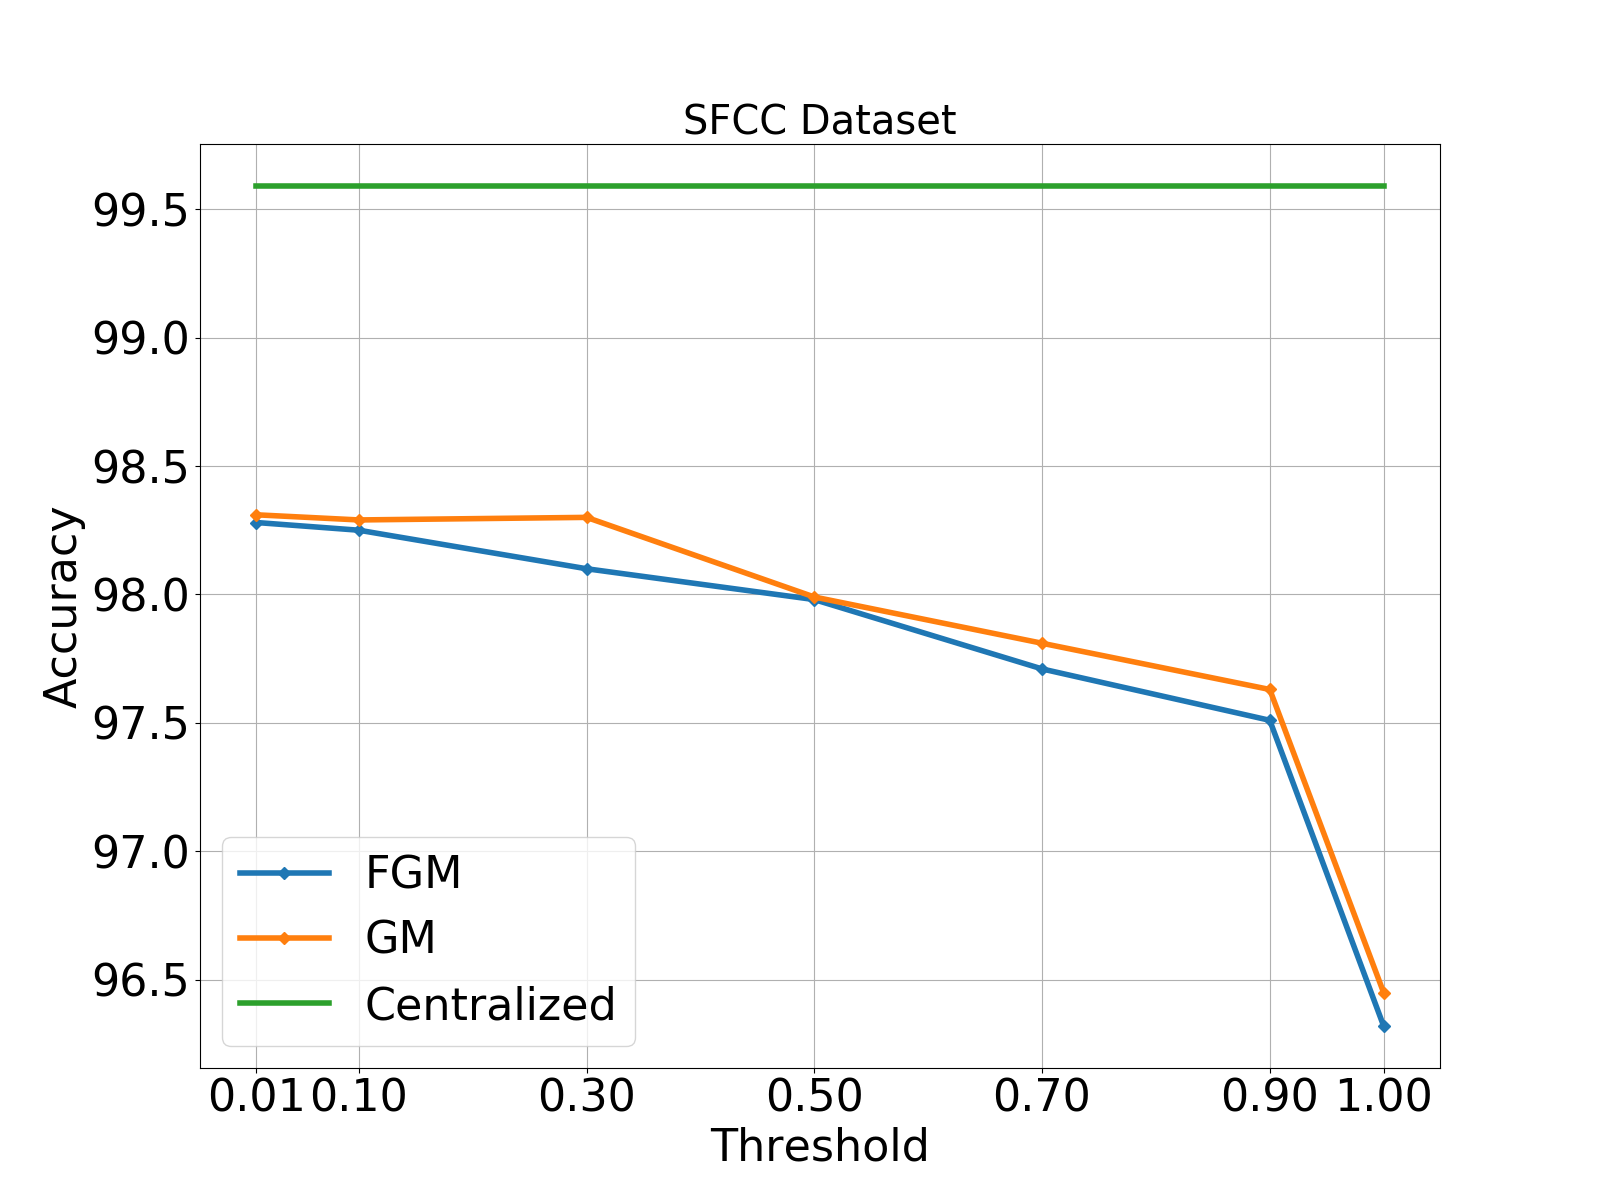
\includegraphics[width=3.9cm,height=3.5cm]{./images/results/sfc-plots/exp_Fig_1_1.png}}
        \subfigure{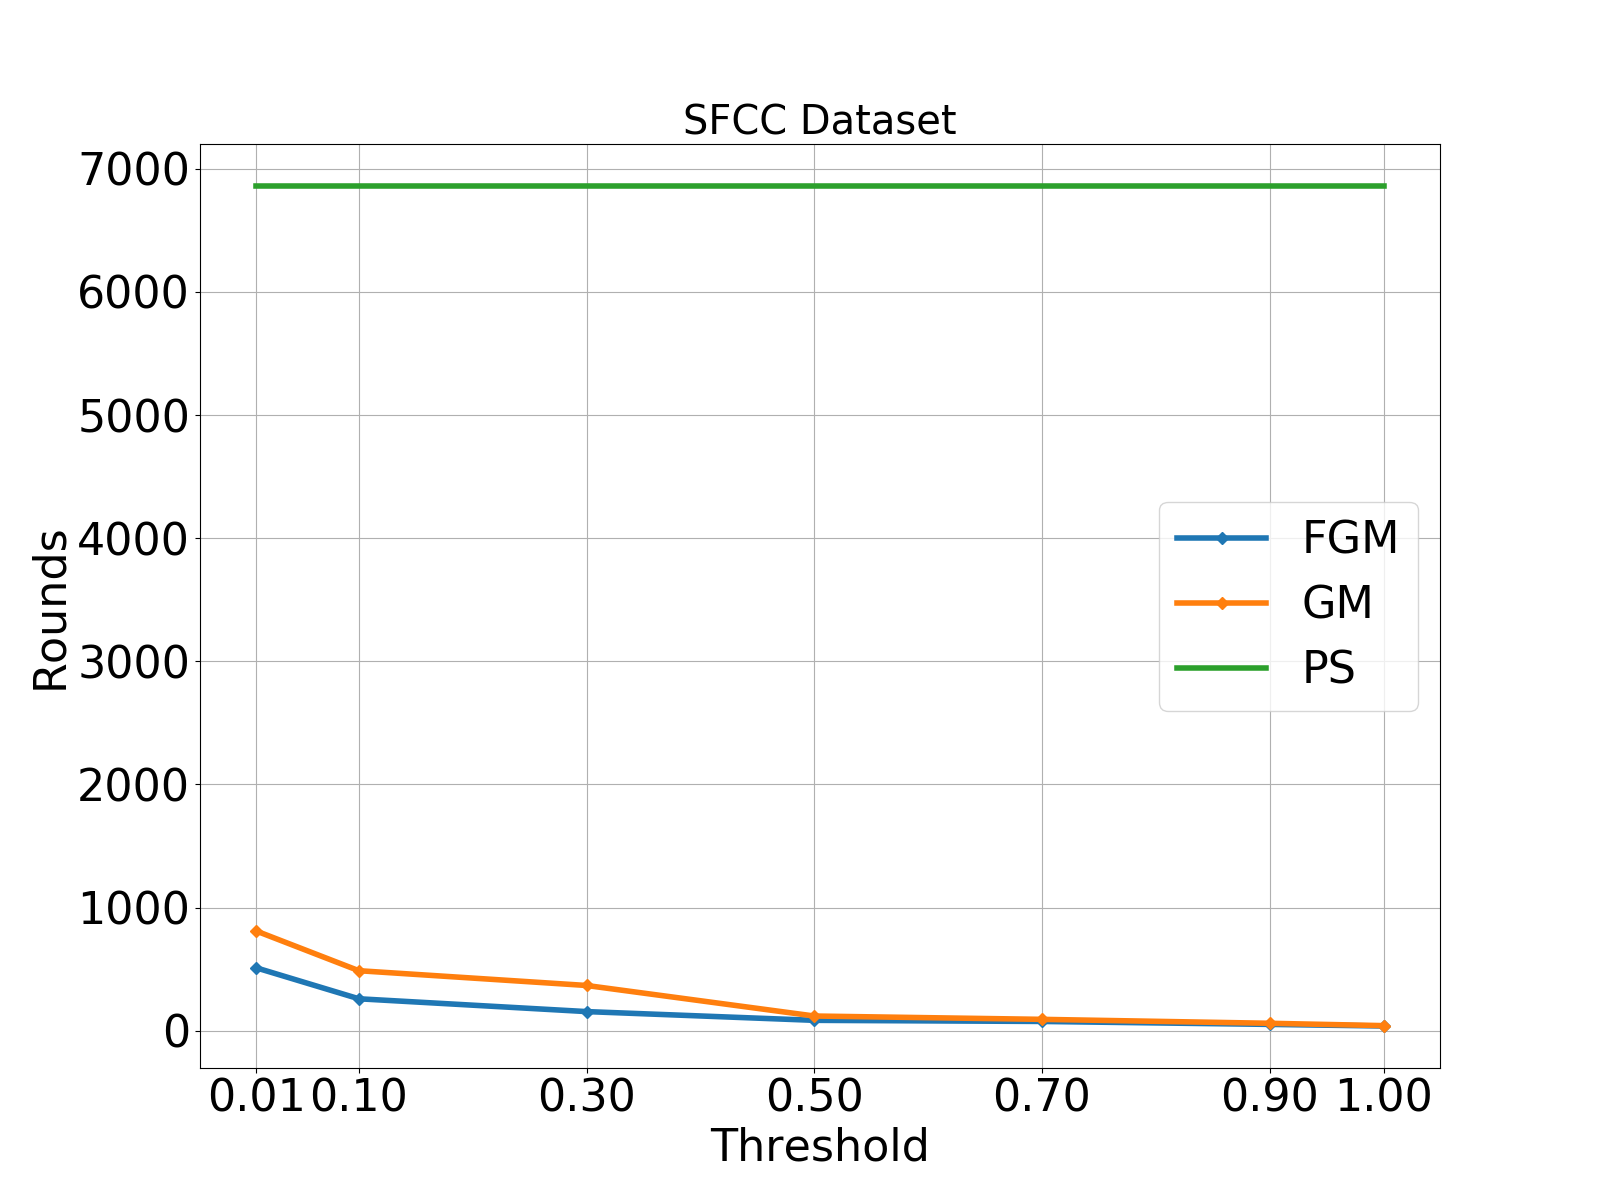
\includegraphics[width=3.9cm,height=3.5cm]{./images/results/sfc-plots/exp_Fig_1_2.png}}
        \subfigure{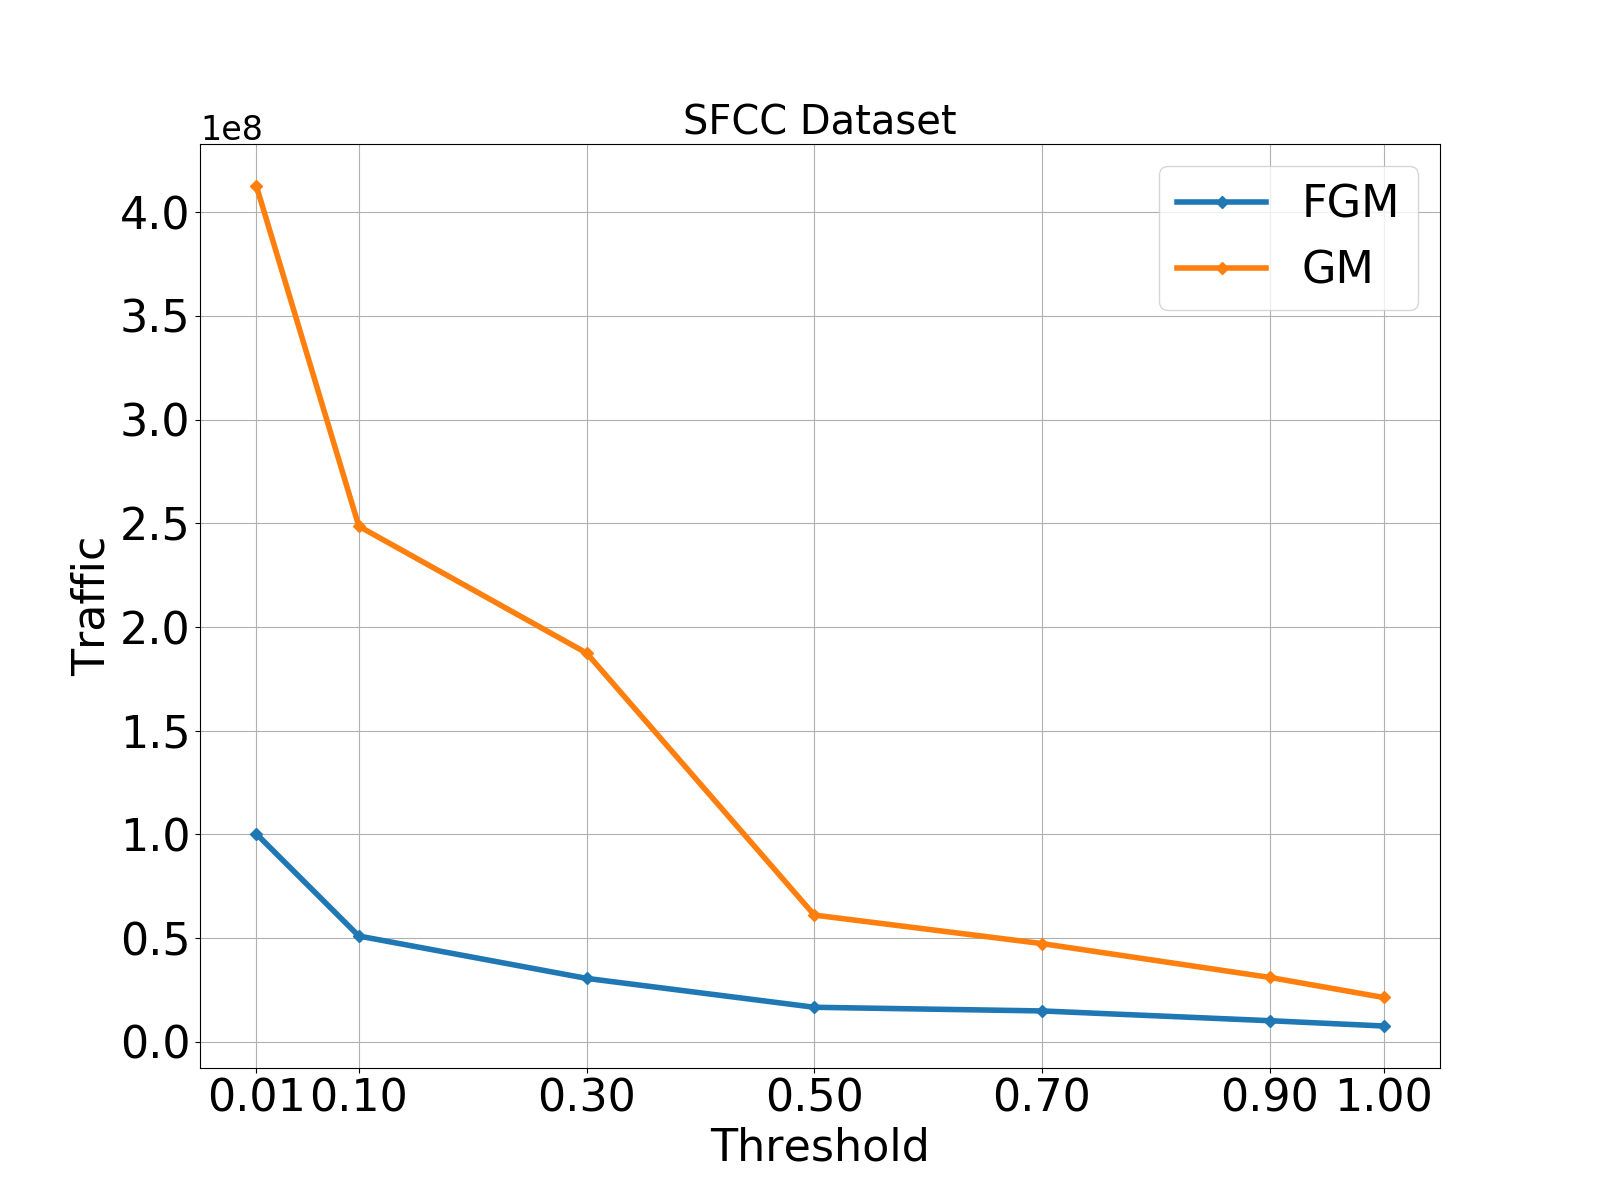
\includegraphics[width=3.9cm,height=3.5cm]{./images/results/sfc-plots/exp_Fig_1_3.png}}
        \subfigure{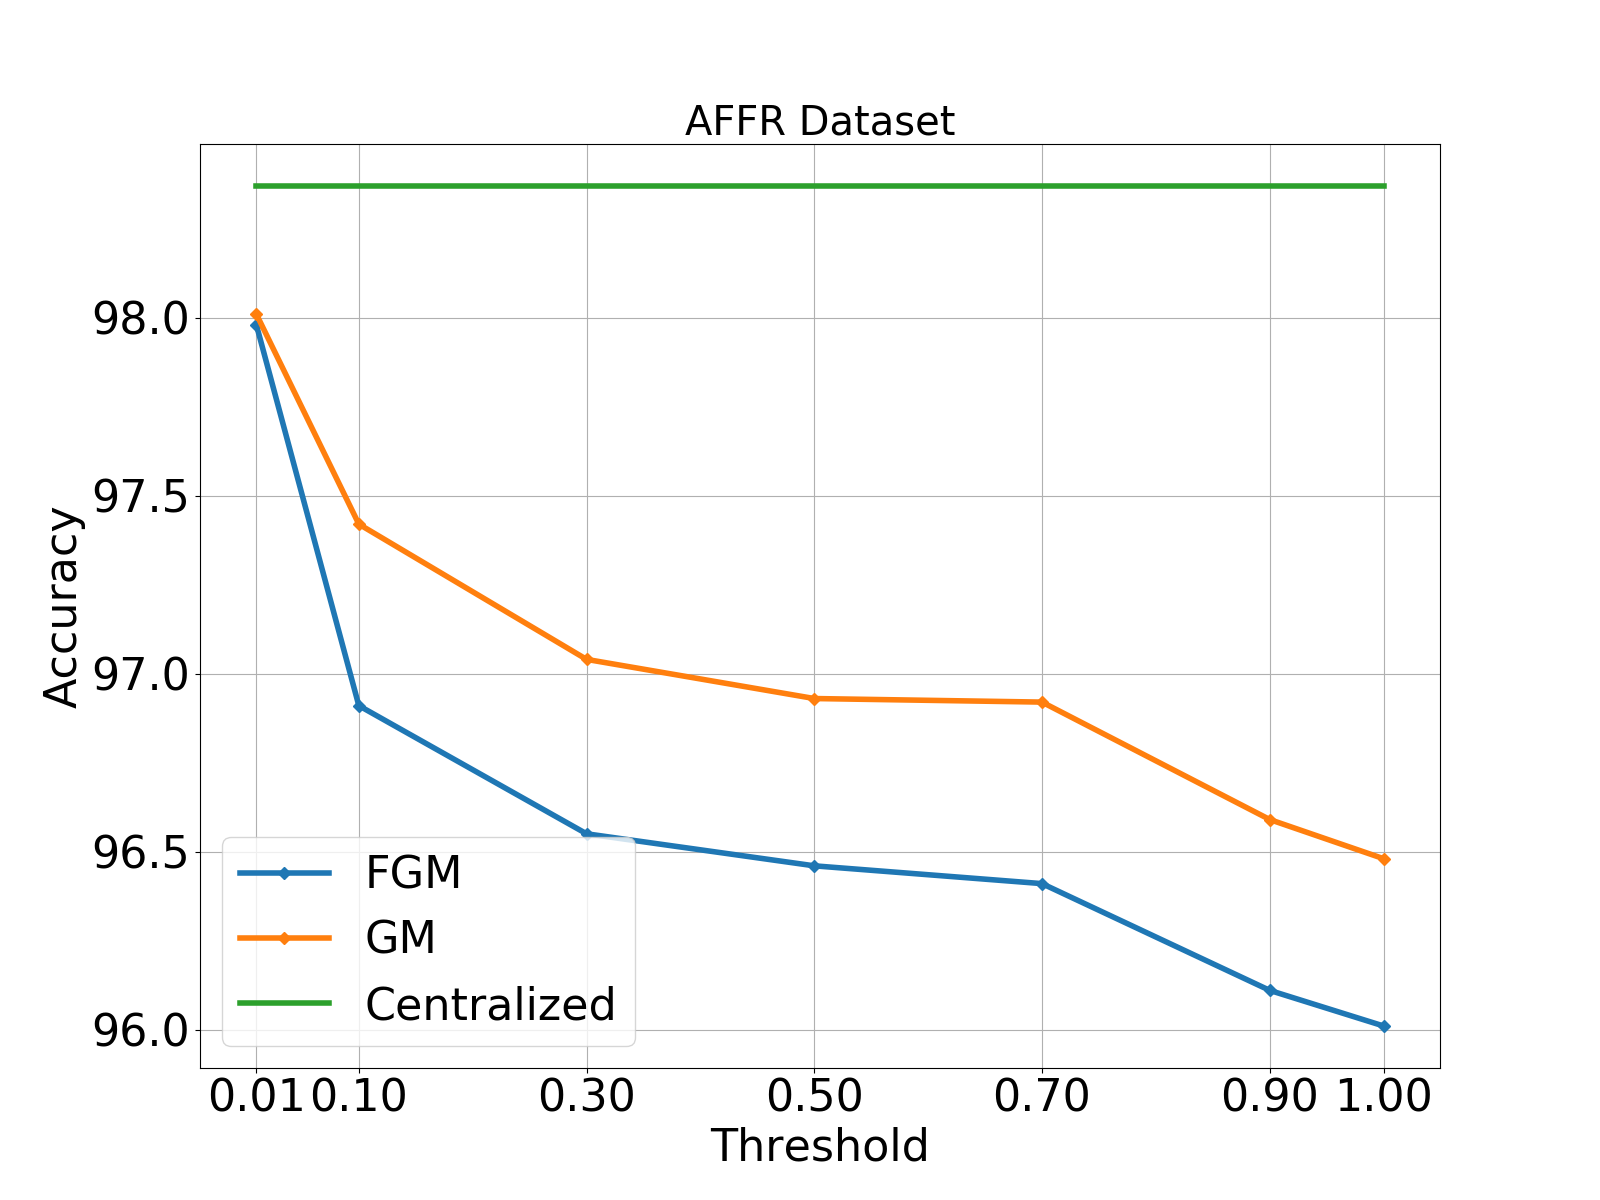
\includegraphics[width=3.9cm,height=3.5cm]{./images/results/amazon-plots/exp_Fig_1_1.png}}
        \subfigure{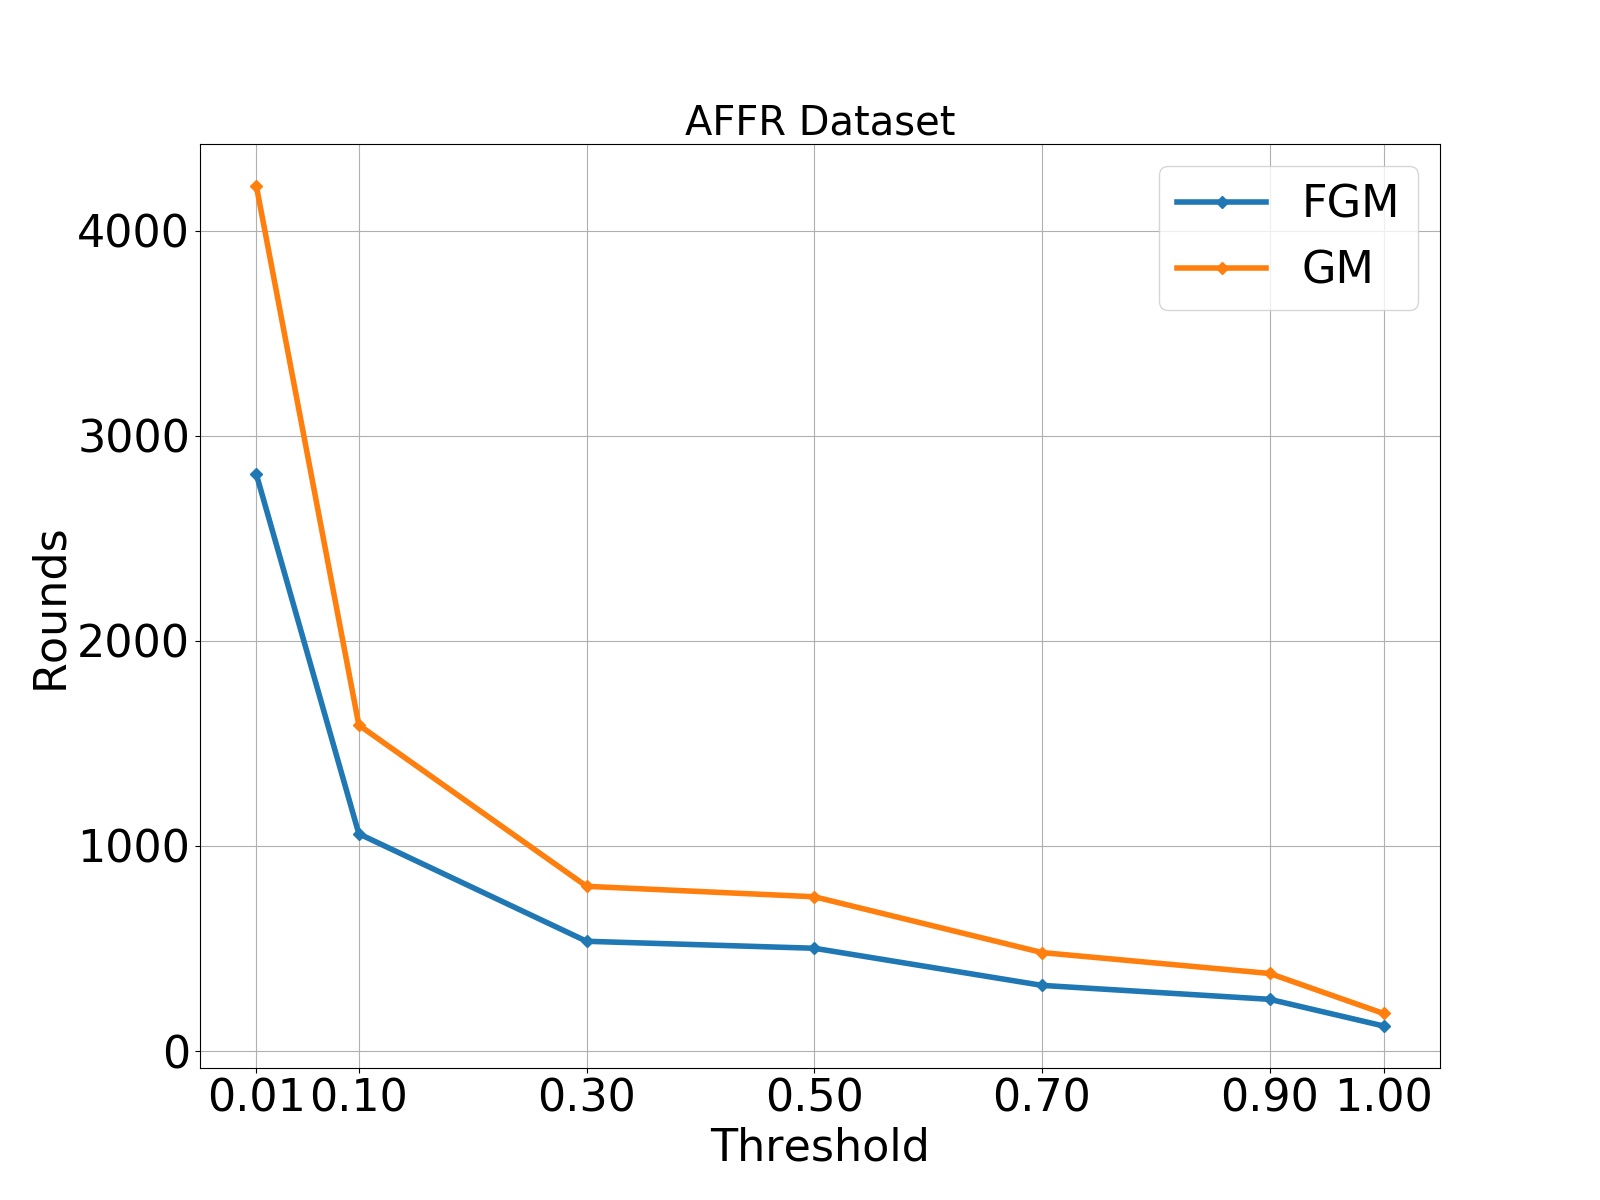
\includegraphics[width=3.9cm,height=3.5cm]{./images/results/amazon-plots/exp_Fig_1_2.png}}
        \subfigure{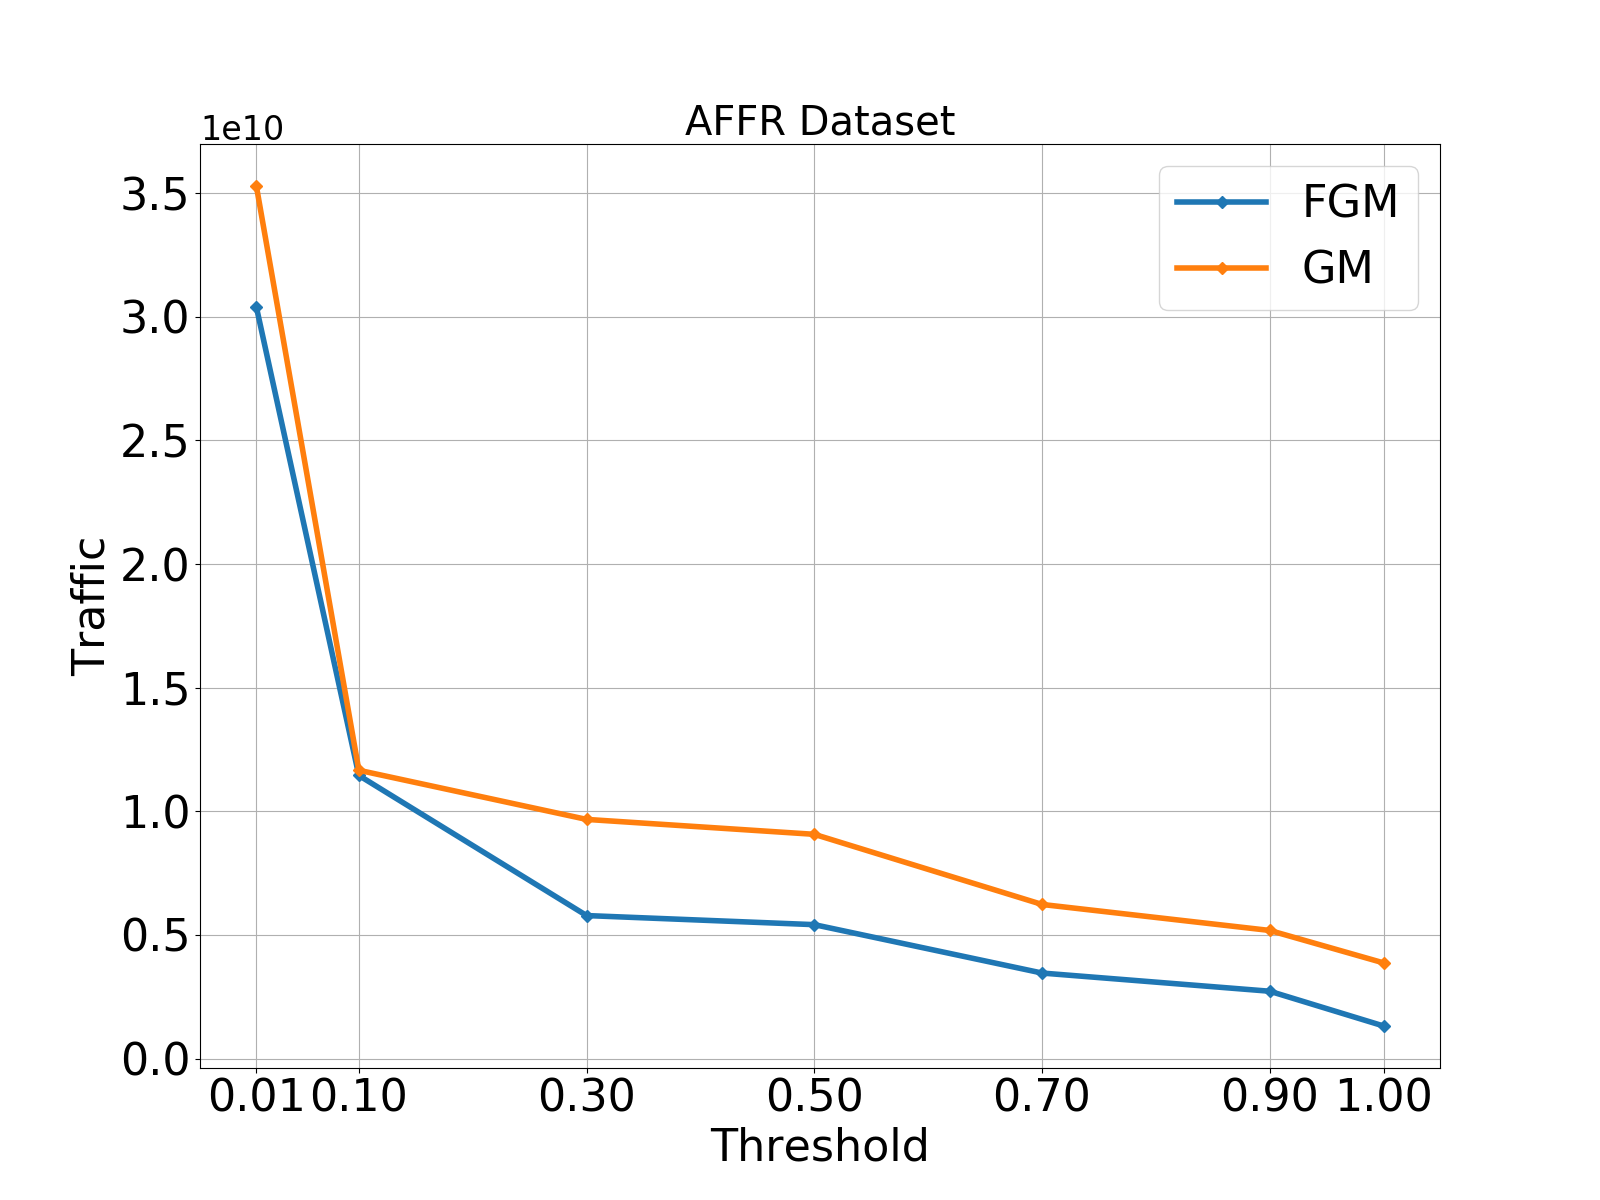
\includegraphics[width=3.9cm,height=3.5cm]{./images/results/amazon-plots/exp_Fig_1_3.png}}
        \label{fig:sfc-amazon-thres}
    \end{figure}
\end{frame}

\begin{frame}{Results (2) - Changing the mini-batch size ($\pmb{|\beta|}$)}
%    \begin{itemize}
%        \item[]{A comment.}
%    \end{itemize}
%    \vspace{-0.4cm}
    \begin{figure}
        \subfigure{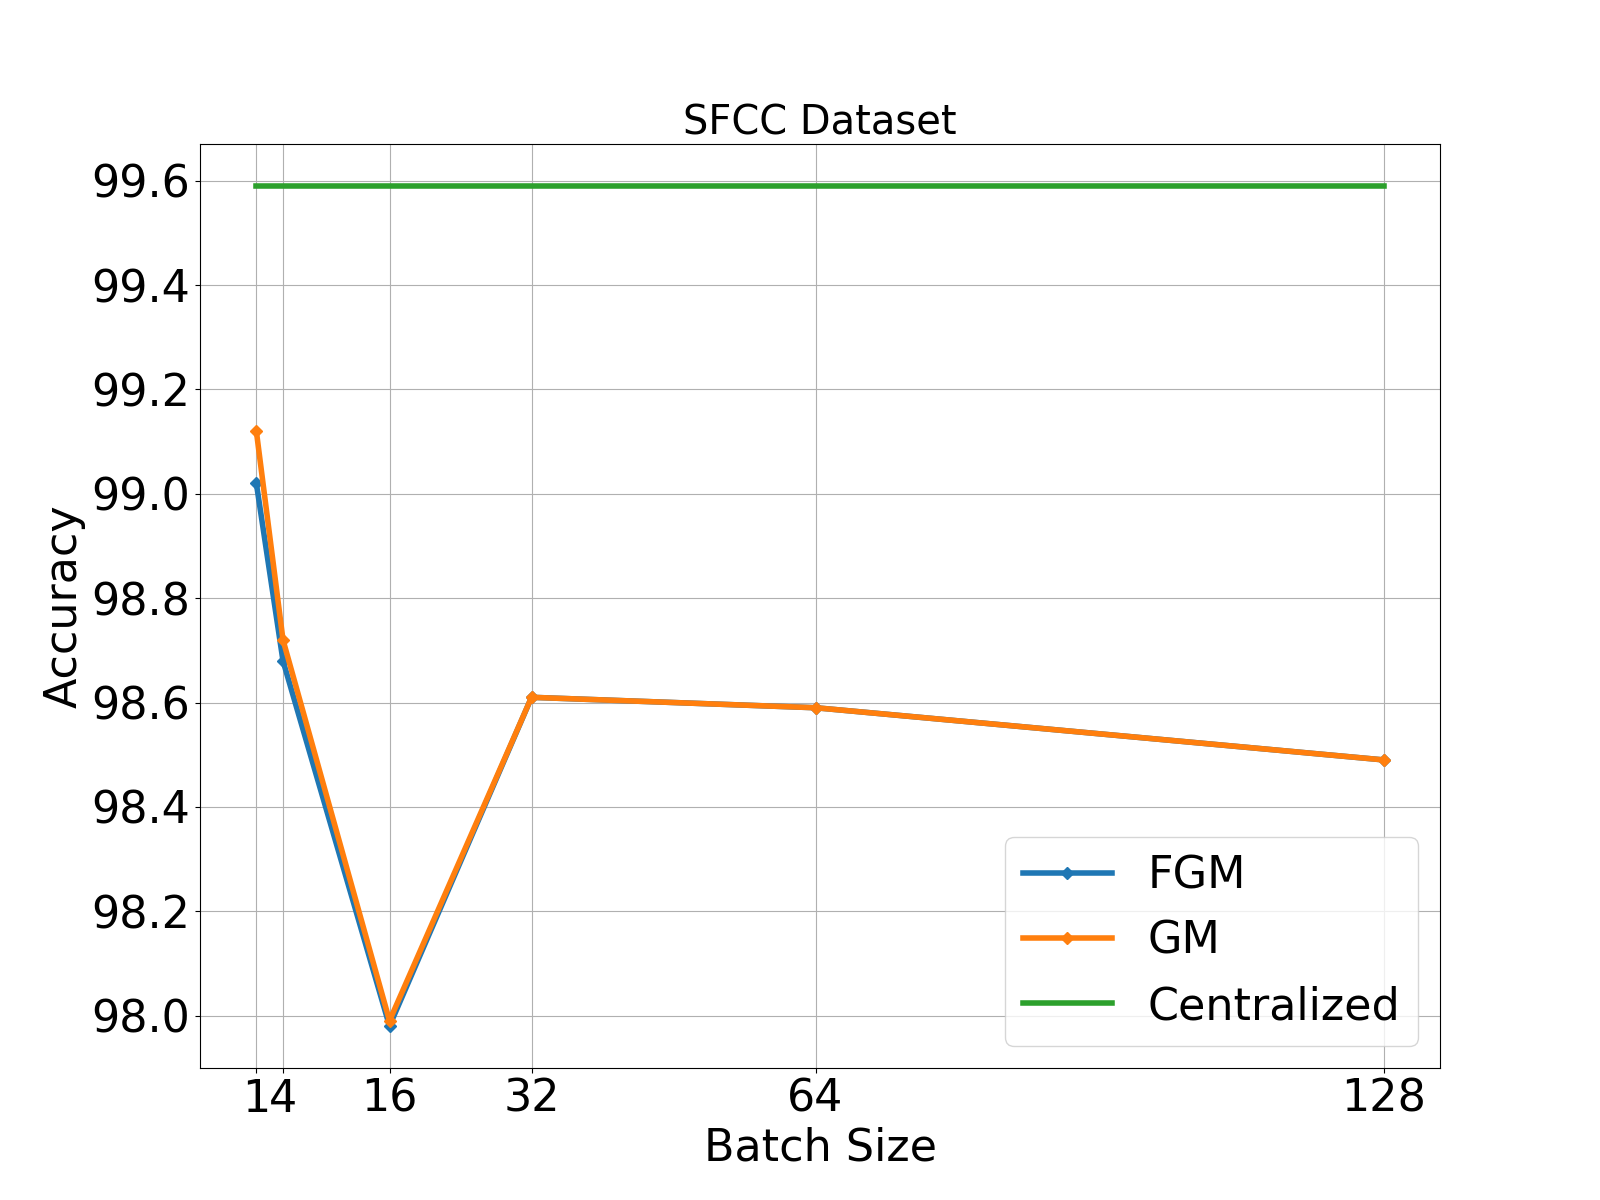
\includegraphics[width=3.9cm,height=3.5cm]{./images/results/sfc-plots/exp_Fig_2_1.png}}
        \subfigure{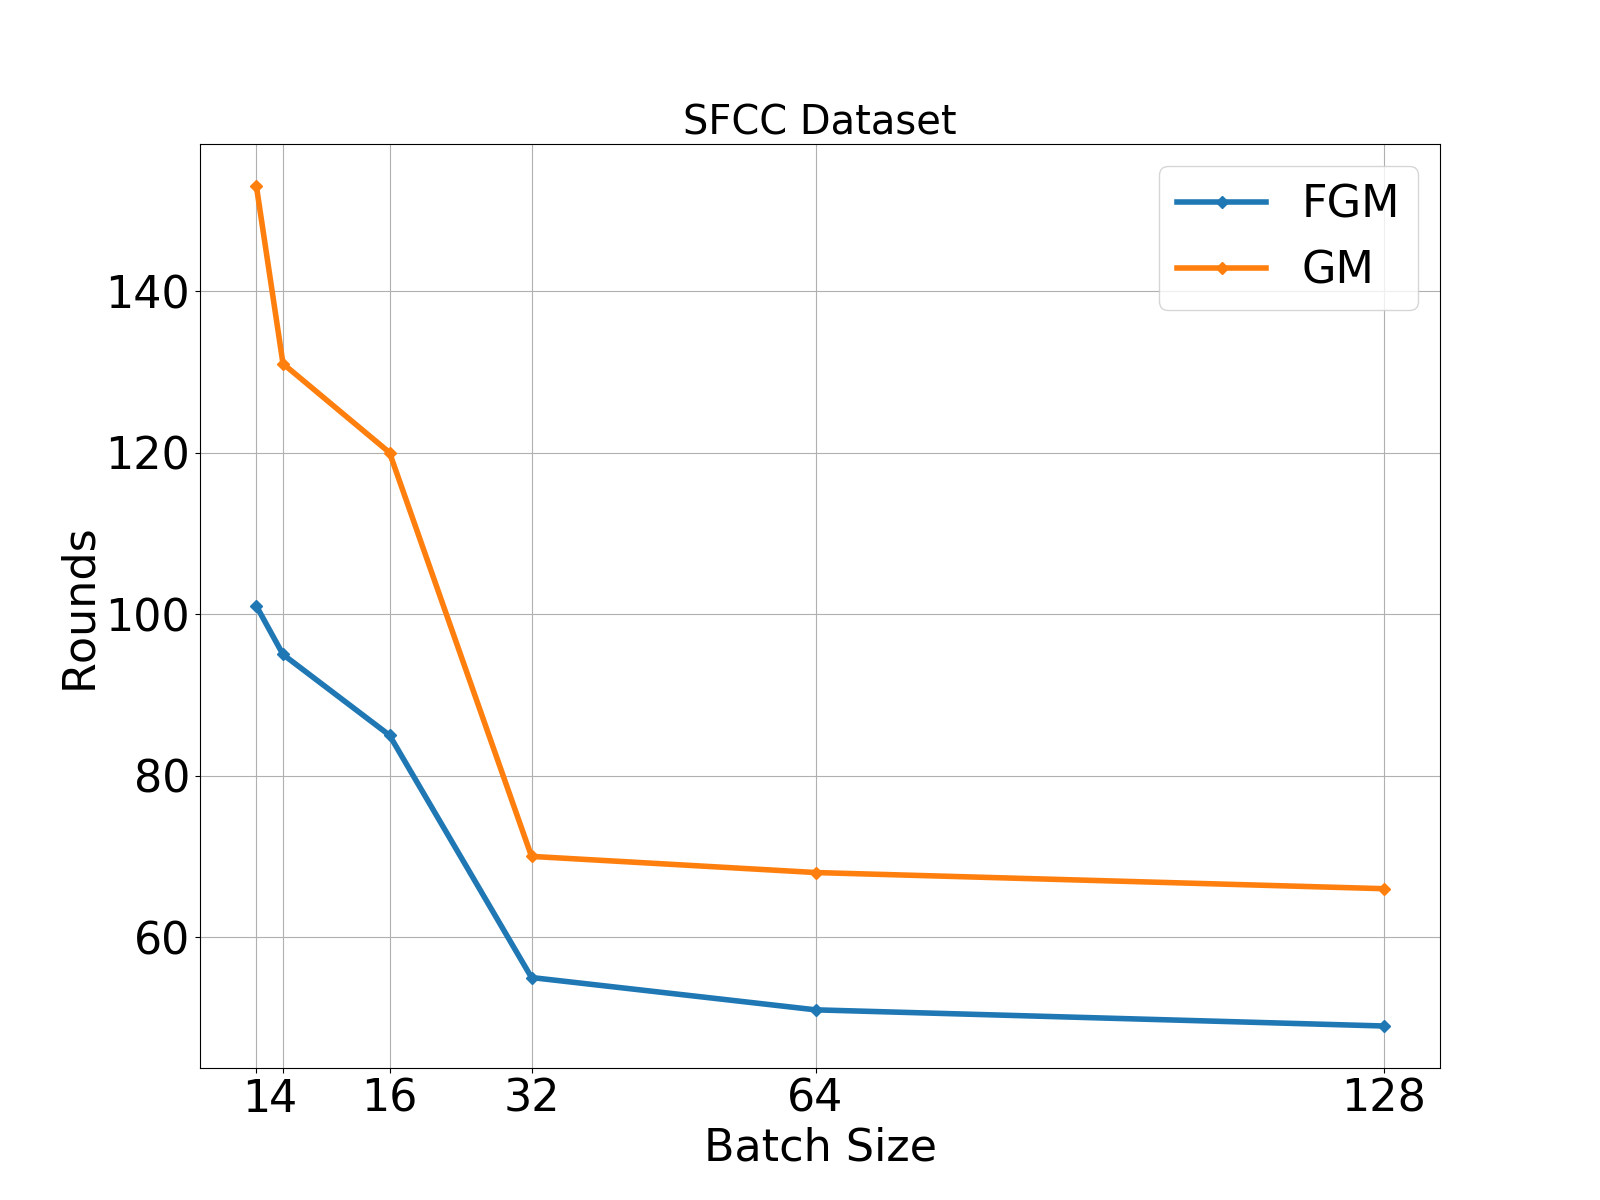
\includegraphics[width=3.9cm,height=3.5cm]{./images/results/sfc-plots/exp_Fig_2_2.png}}
        \subfigure{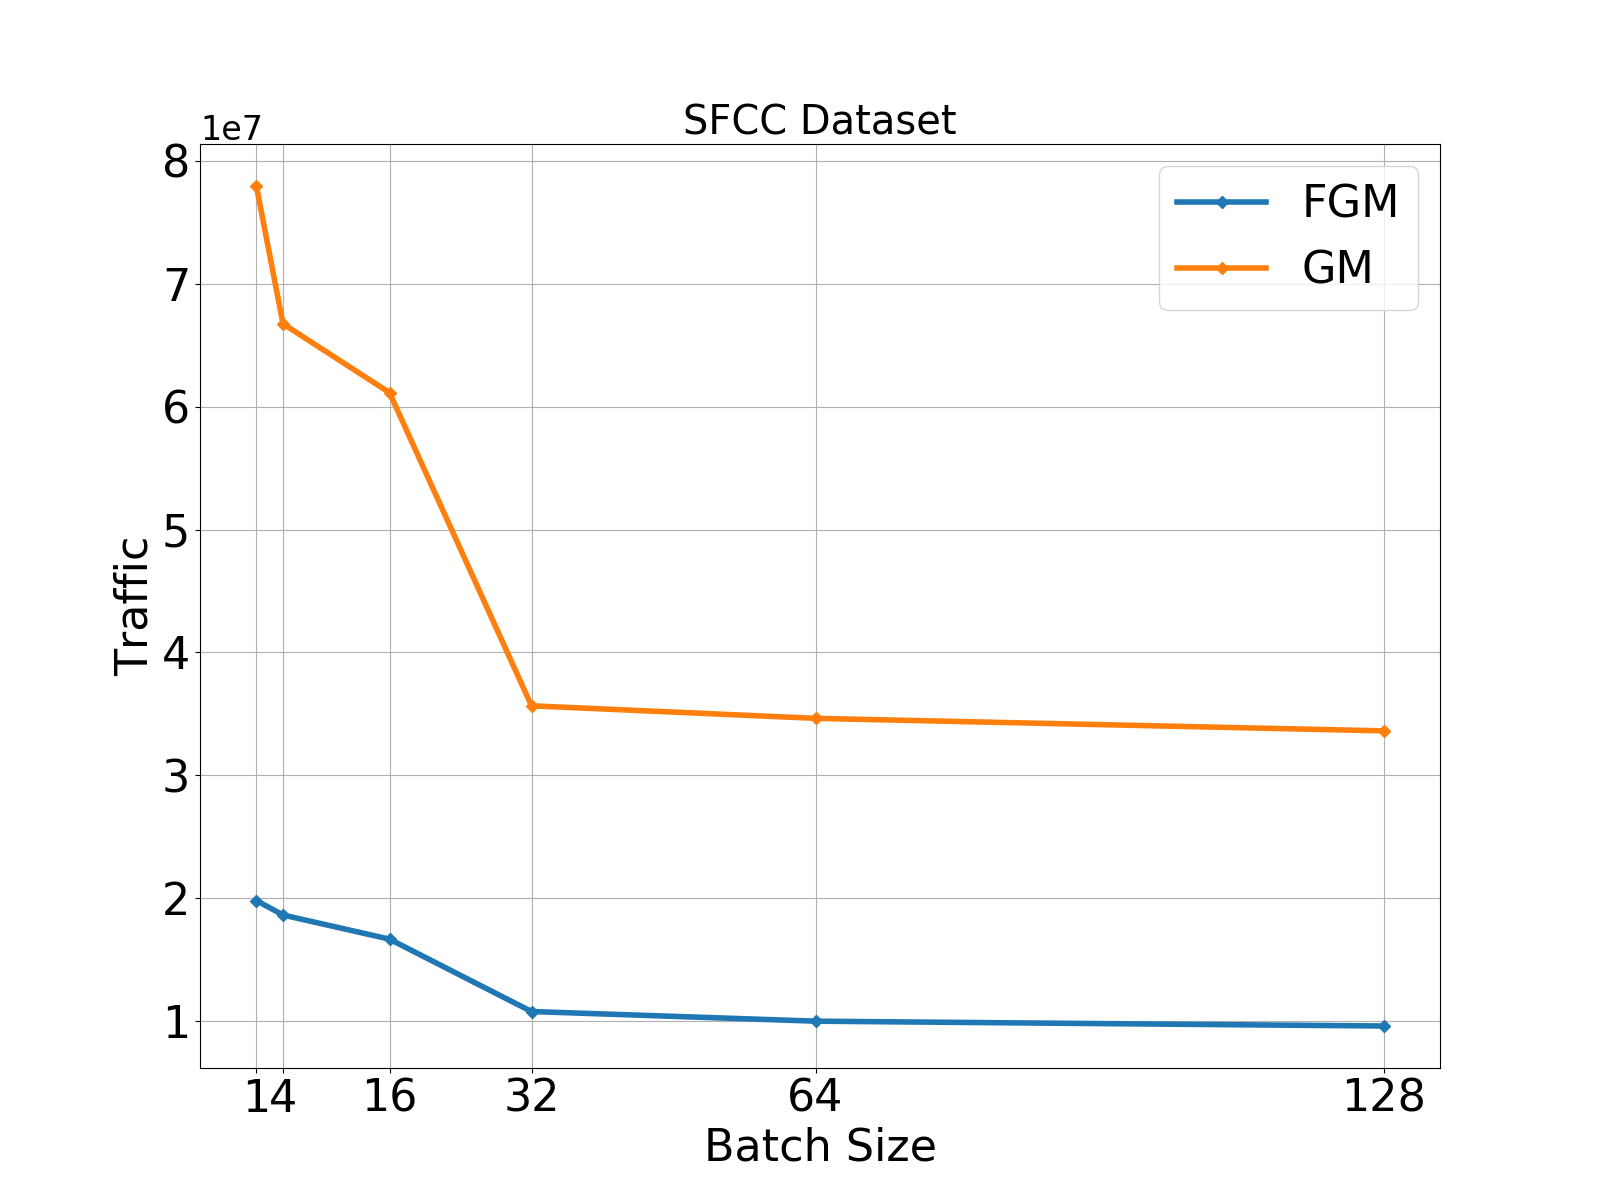
\includegraphics[width=3.9cm,height=3.5cm]{./images/results/sfc-plots/exp_Fig_2_3.png}}
        \subfigure{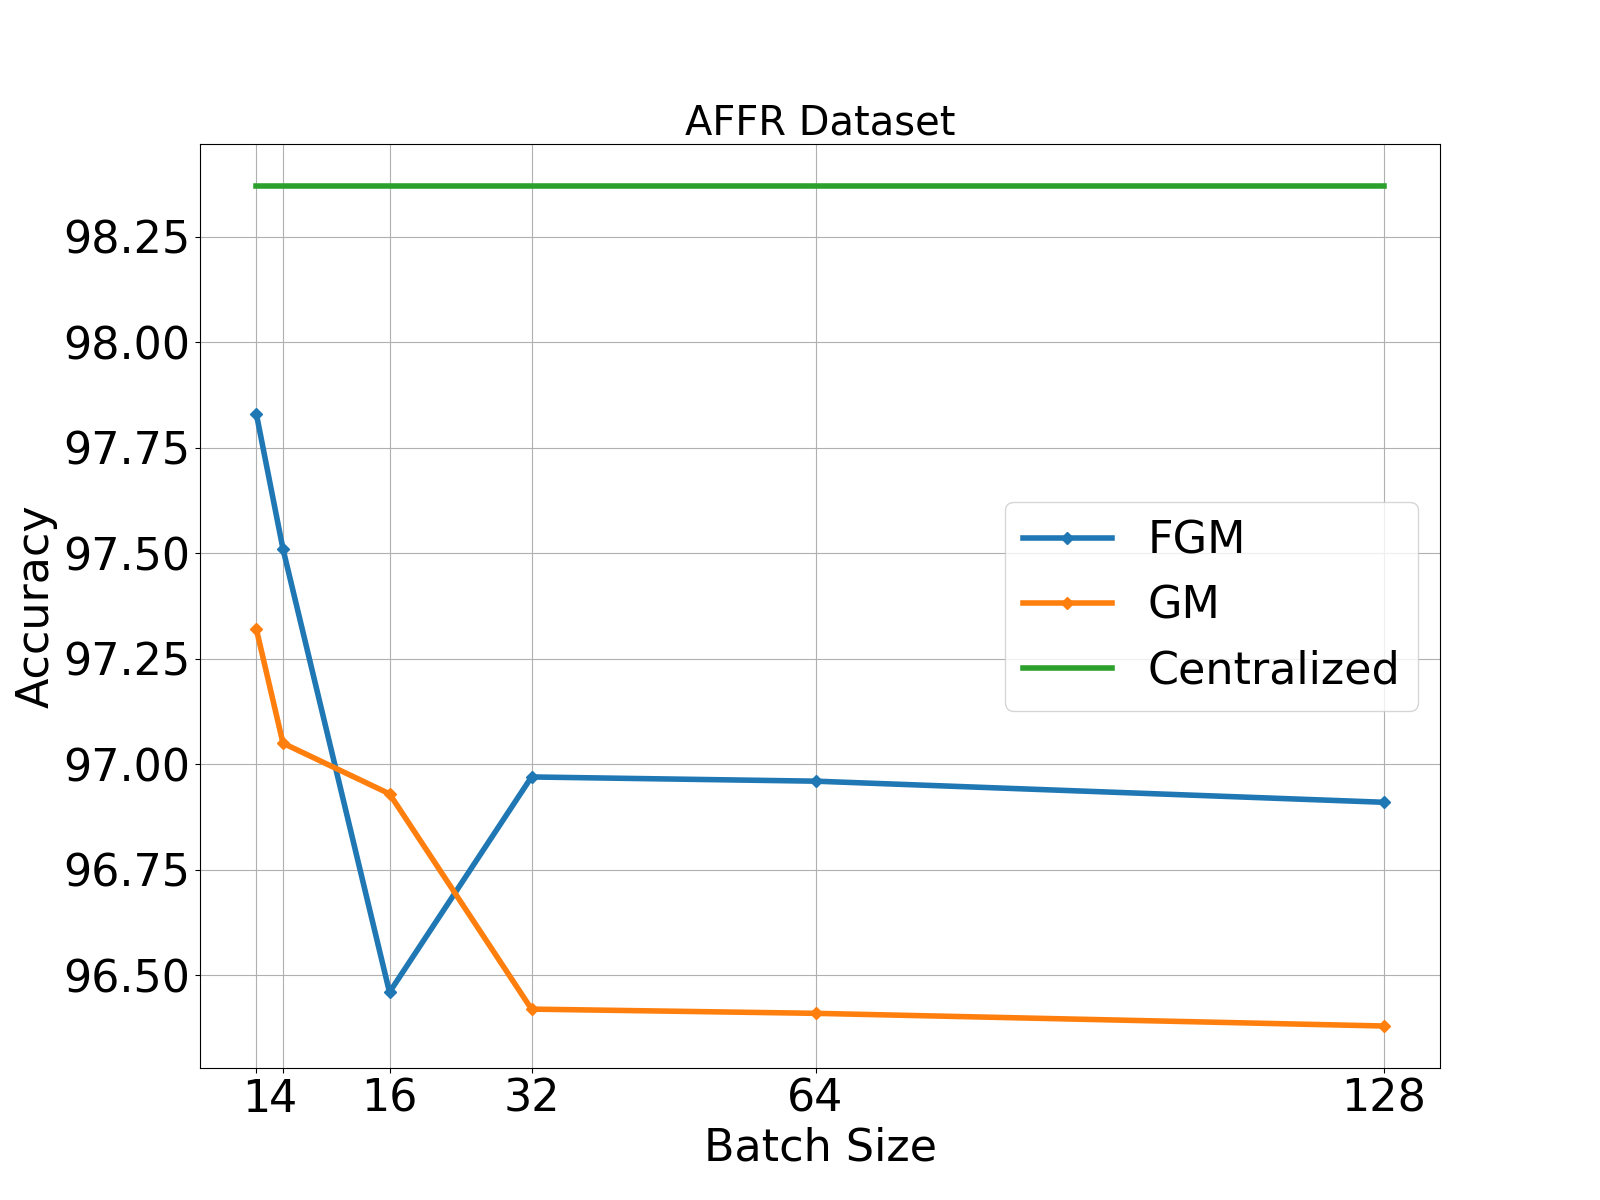
\includegraphics[width=3.9cm,height=3.5cm]{./images/results/amazon-plots/exp_Fig_2_1.png}}
        \subfigure{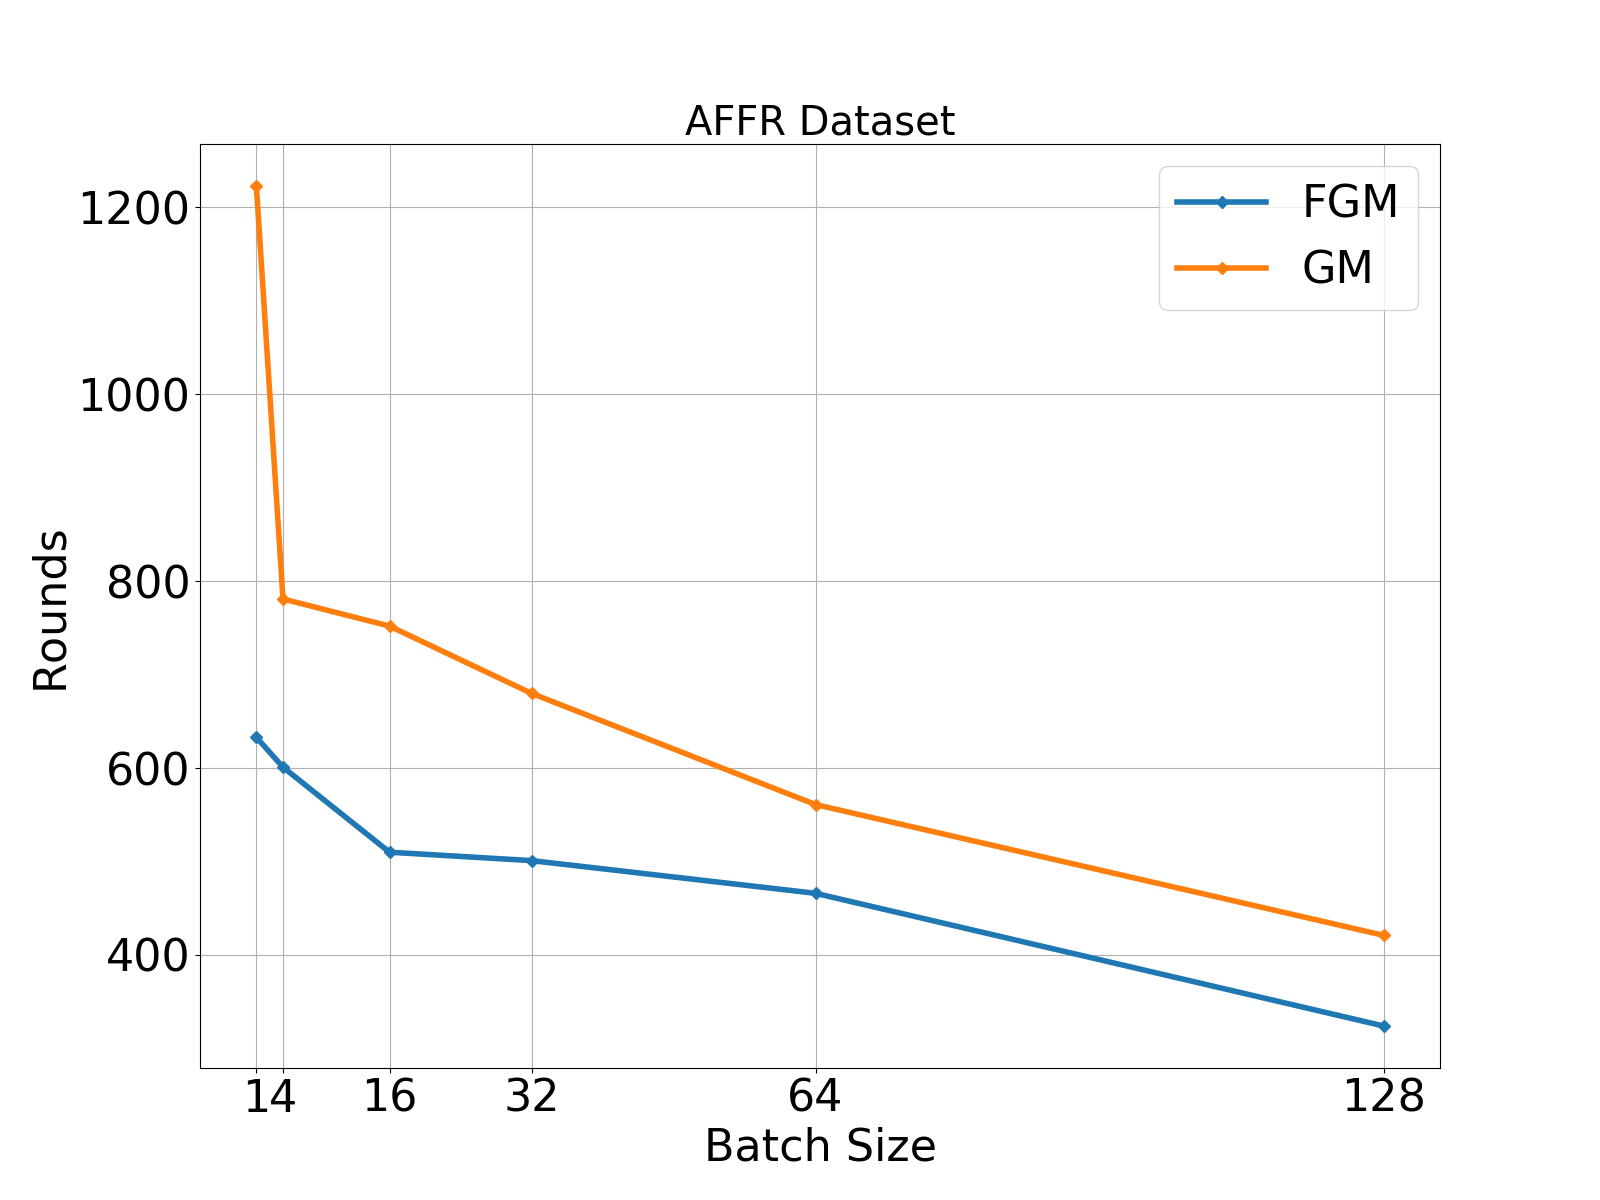
\includegraphics[width=3.9cm,height=3.5cm]{./images/results/amazon-plots/exp_Fig_2_2.png}}
        \subfigure{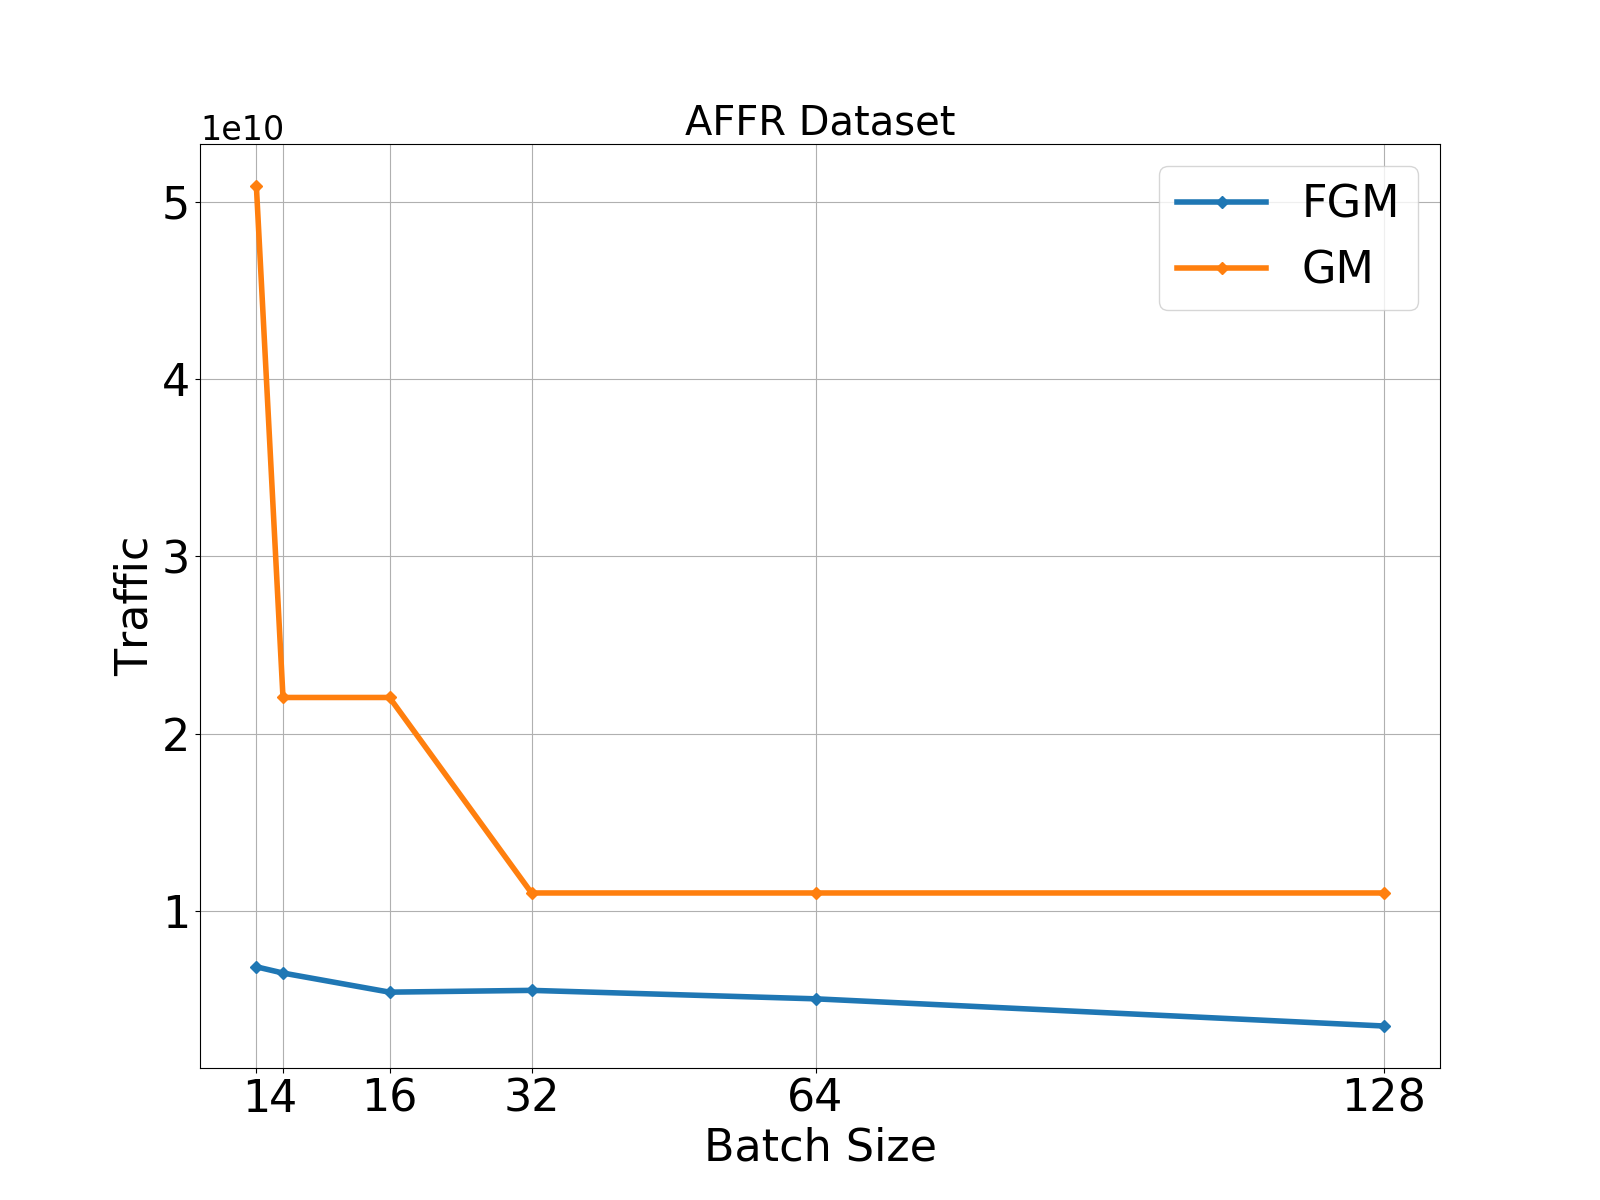
\includegraphics[width=3.9cm,height=3.5cm]{./images/results/amazon-plots/exp_Fig_2_3.png}}
        \label{fig:sfc-amazon-bs}
    \end{figure}
\end{frame}

\begin{frame}{Results (3) - Changing the number of workers ($\pmb{n}$)}
%    \begin{itemize}
%        \item[]{A comment.}
%    \end{itemize}
%    \vspace{-0.4cm}
    \begin{figure}
        \subfigure{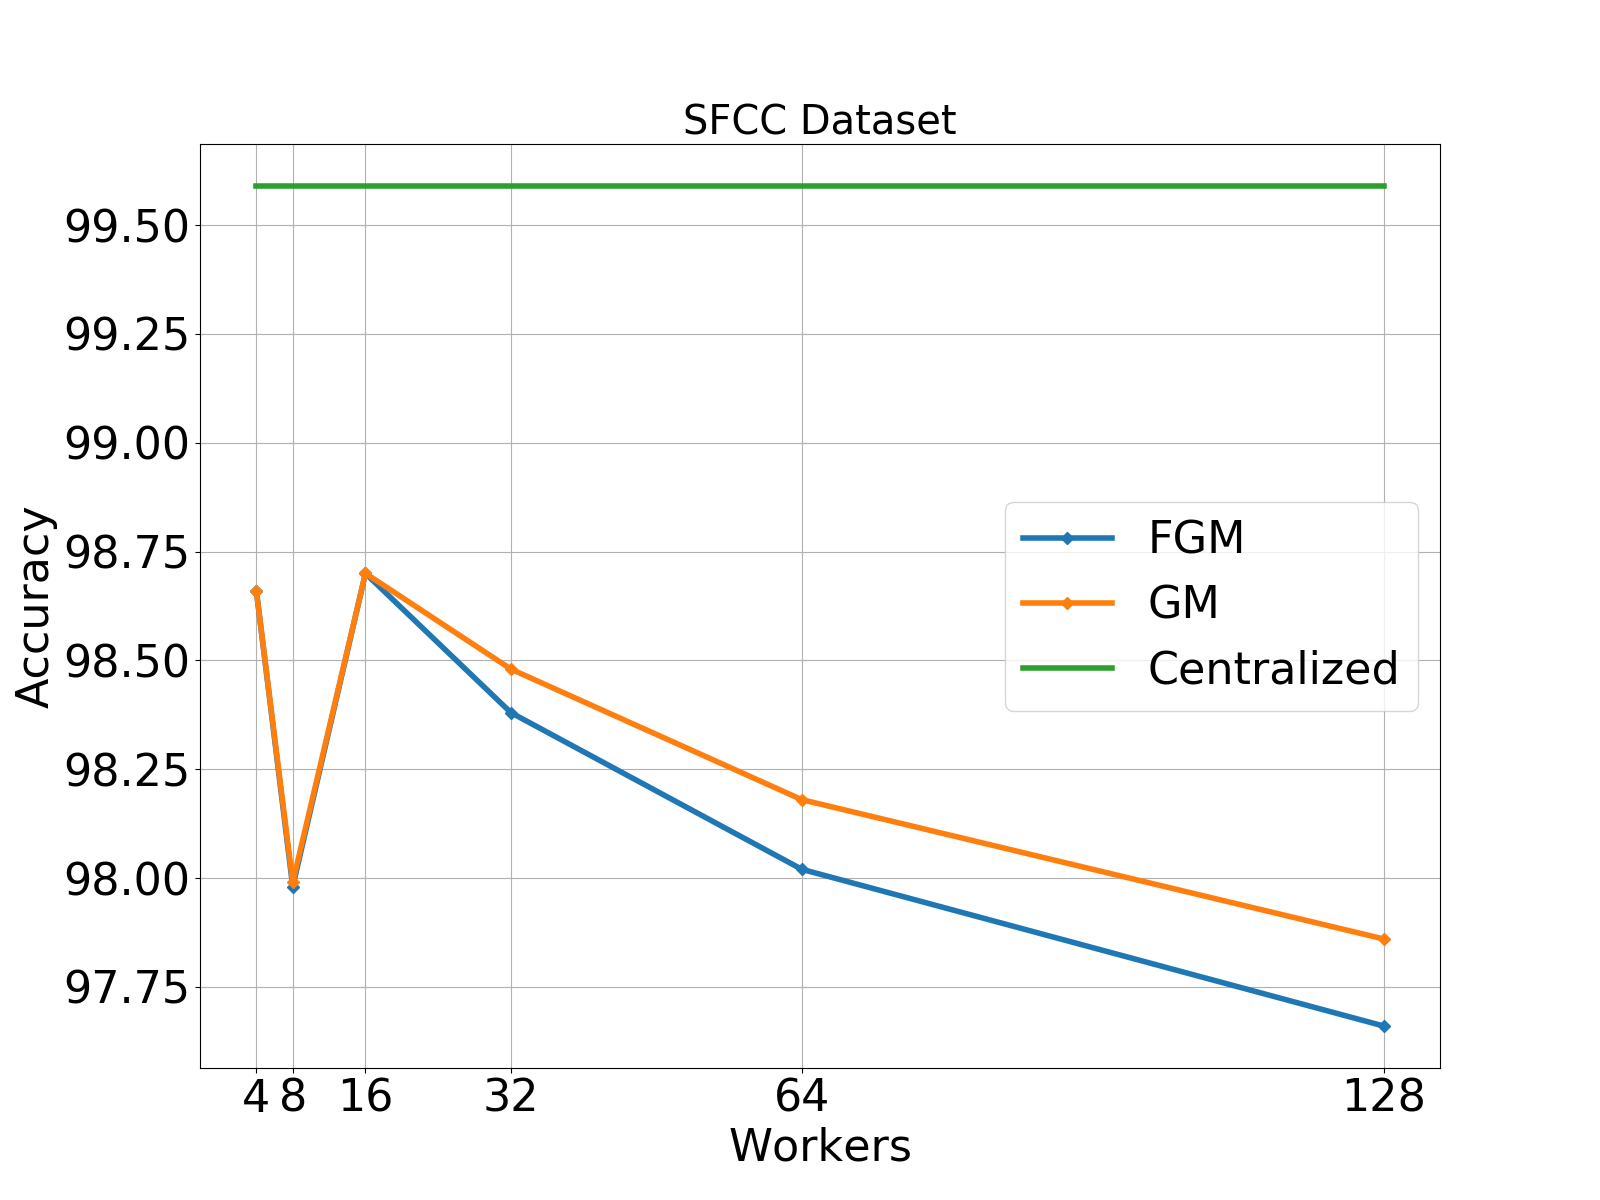
\includegraphics[width=3.9cm,height=3.5cm]{./images/results/sfc-plots/exp_Fig_3_1.png}}
        \subfigure{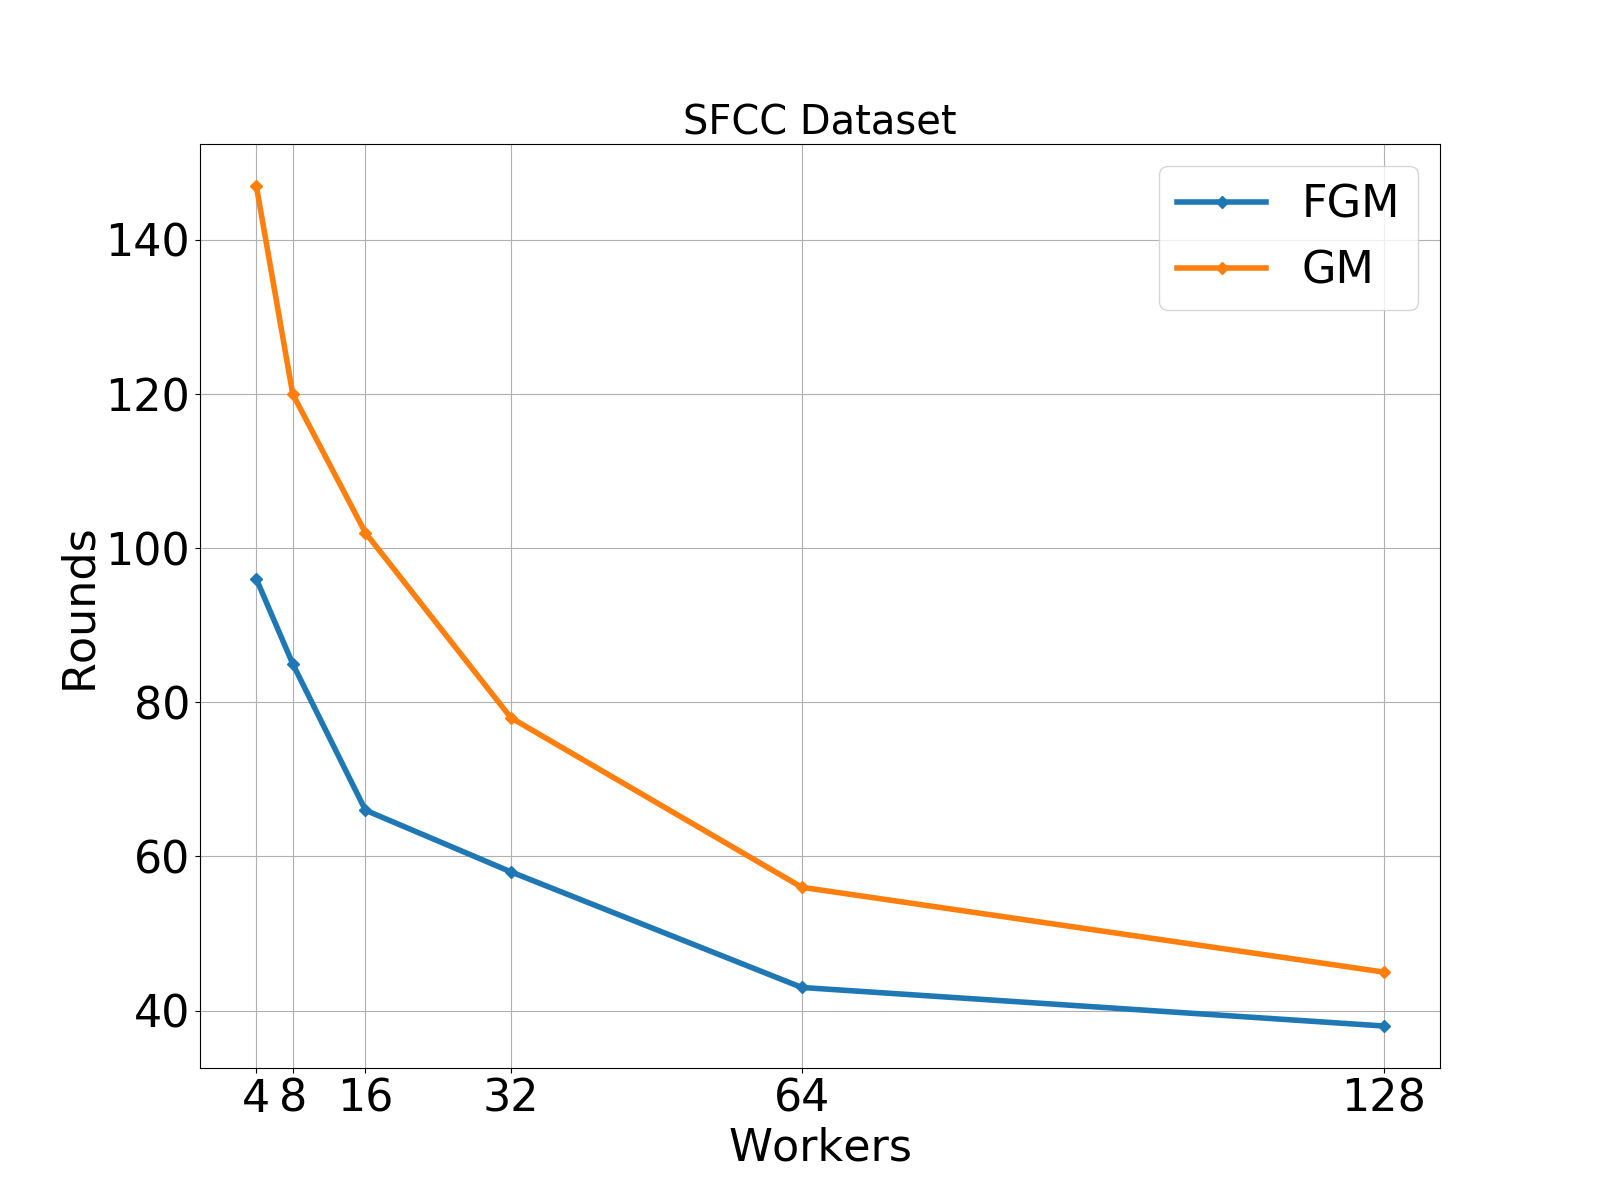
\includegraphics[width=3.9cm,height=3.5cm]{./images/results/sfc-plots/exp_Fig_3_2.png}}
        \subfigure{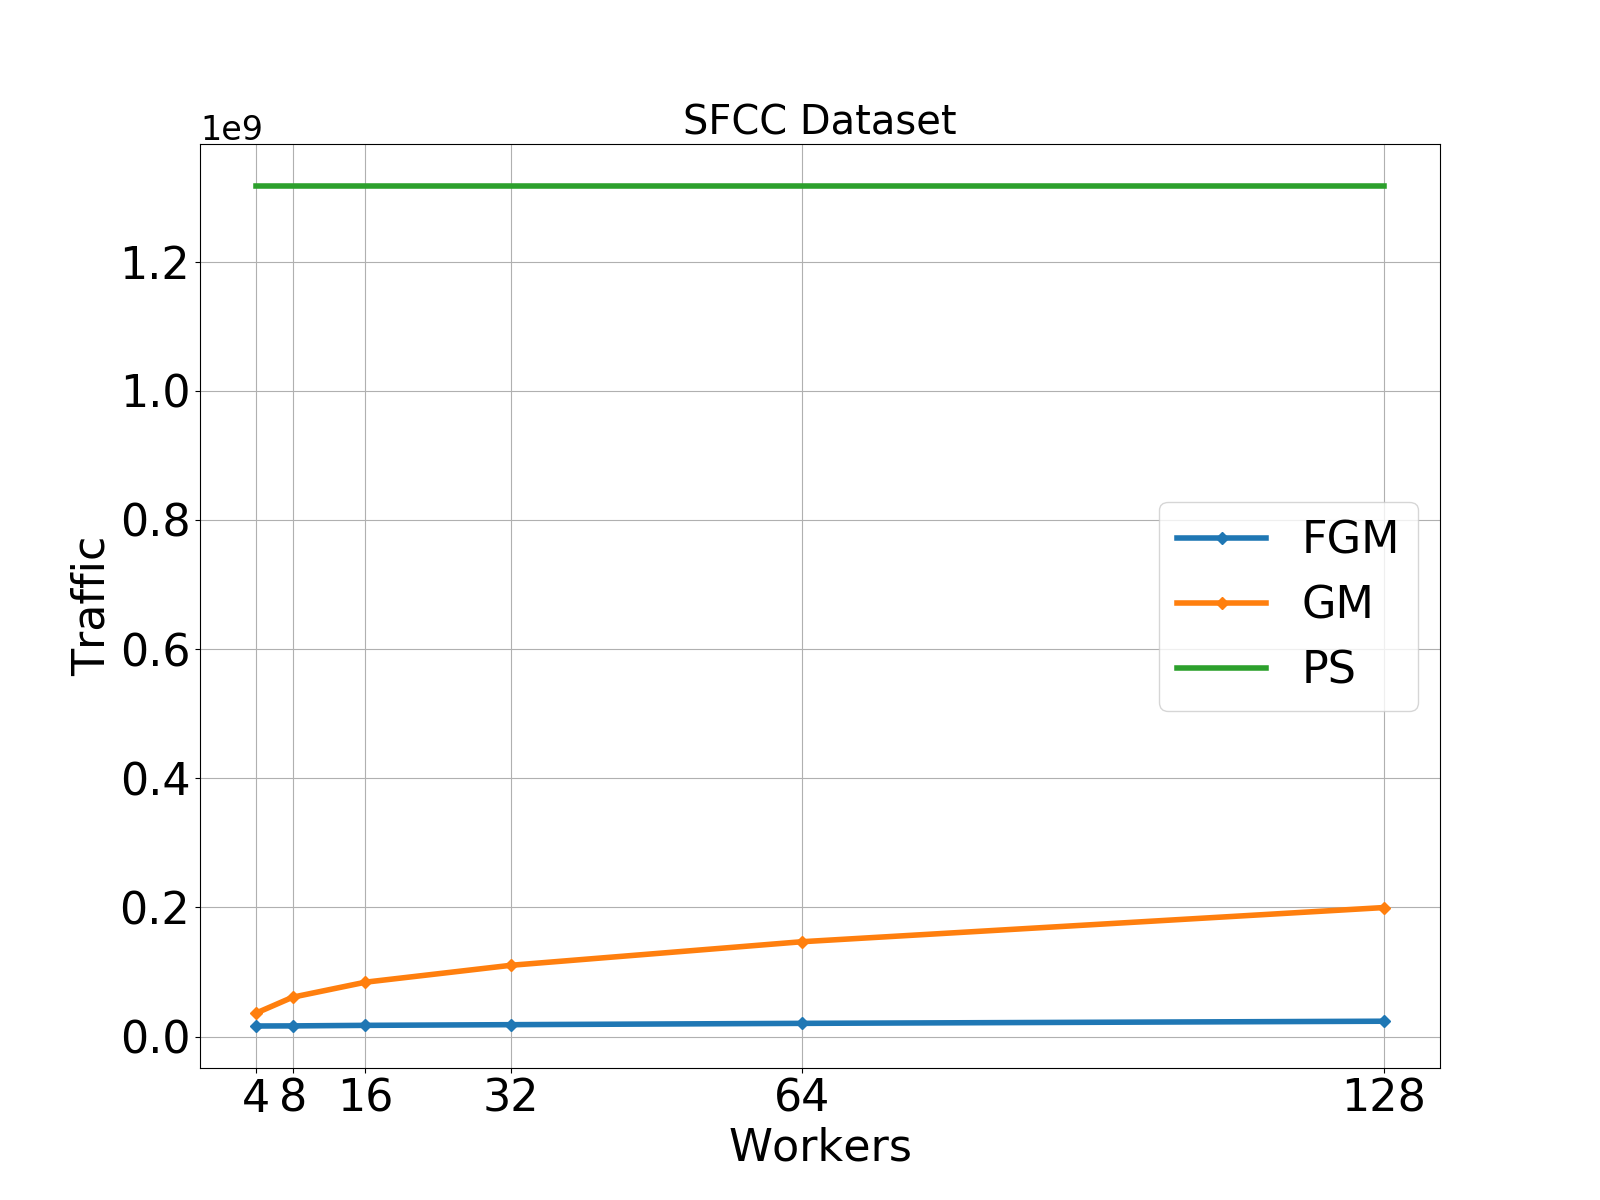
\includegraphics[width=3.9cm,height=3.5cm]{./images/results/sfc-plots/exp_Fig_3_3.png}}
        \subfigure{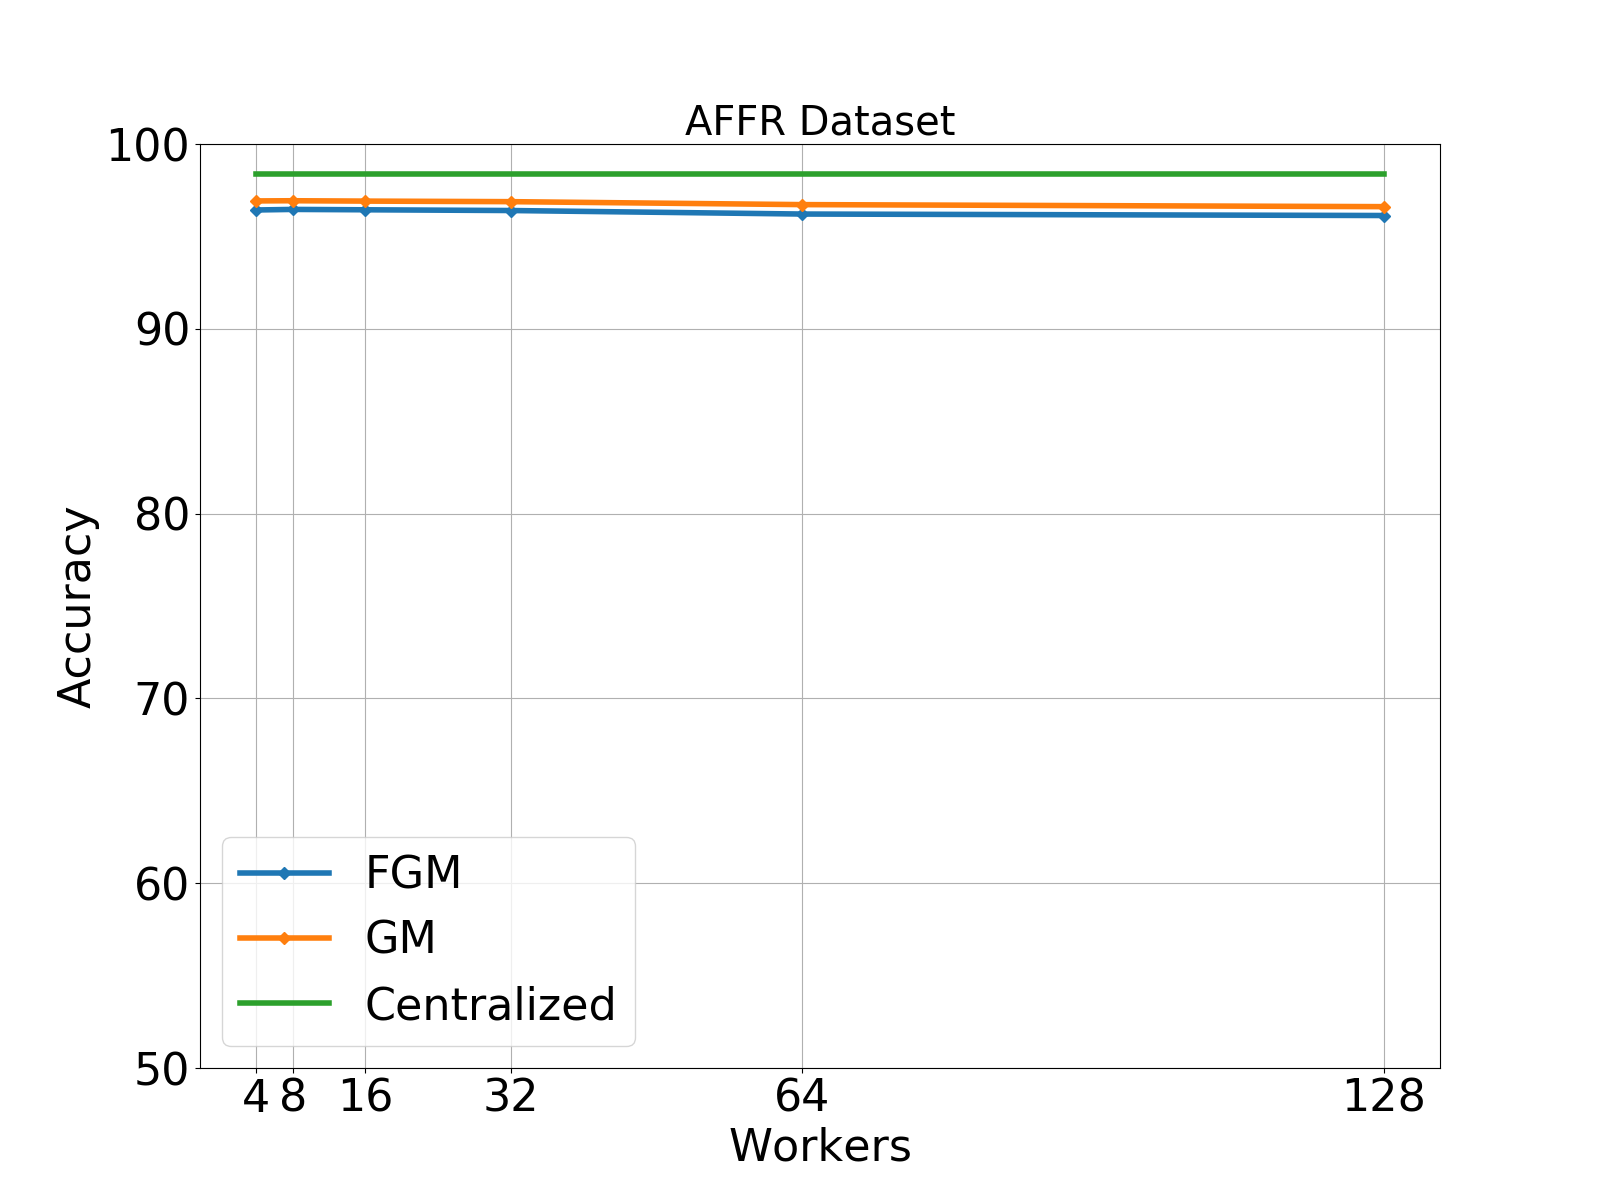
\includegraphics[width=3.9cm,height=3.5cm]{./images/results/amazon-plots/exp_Fig_3_1.png}}
        \subfigure{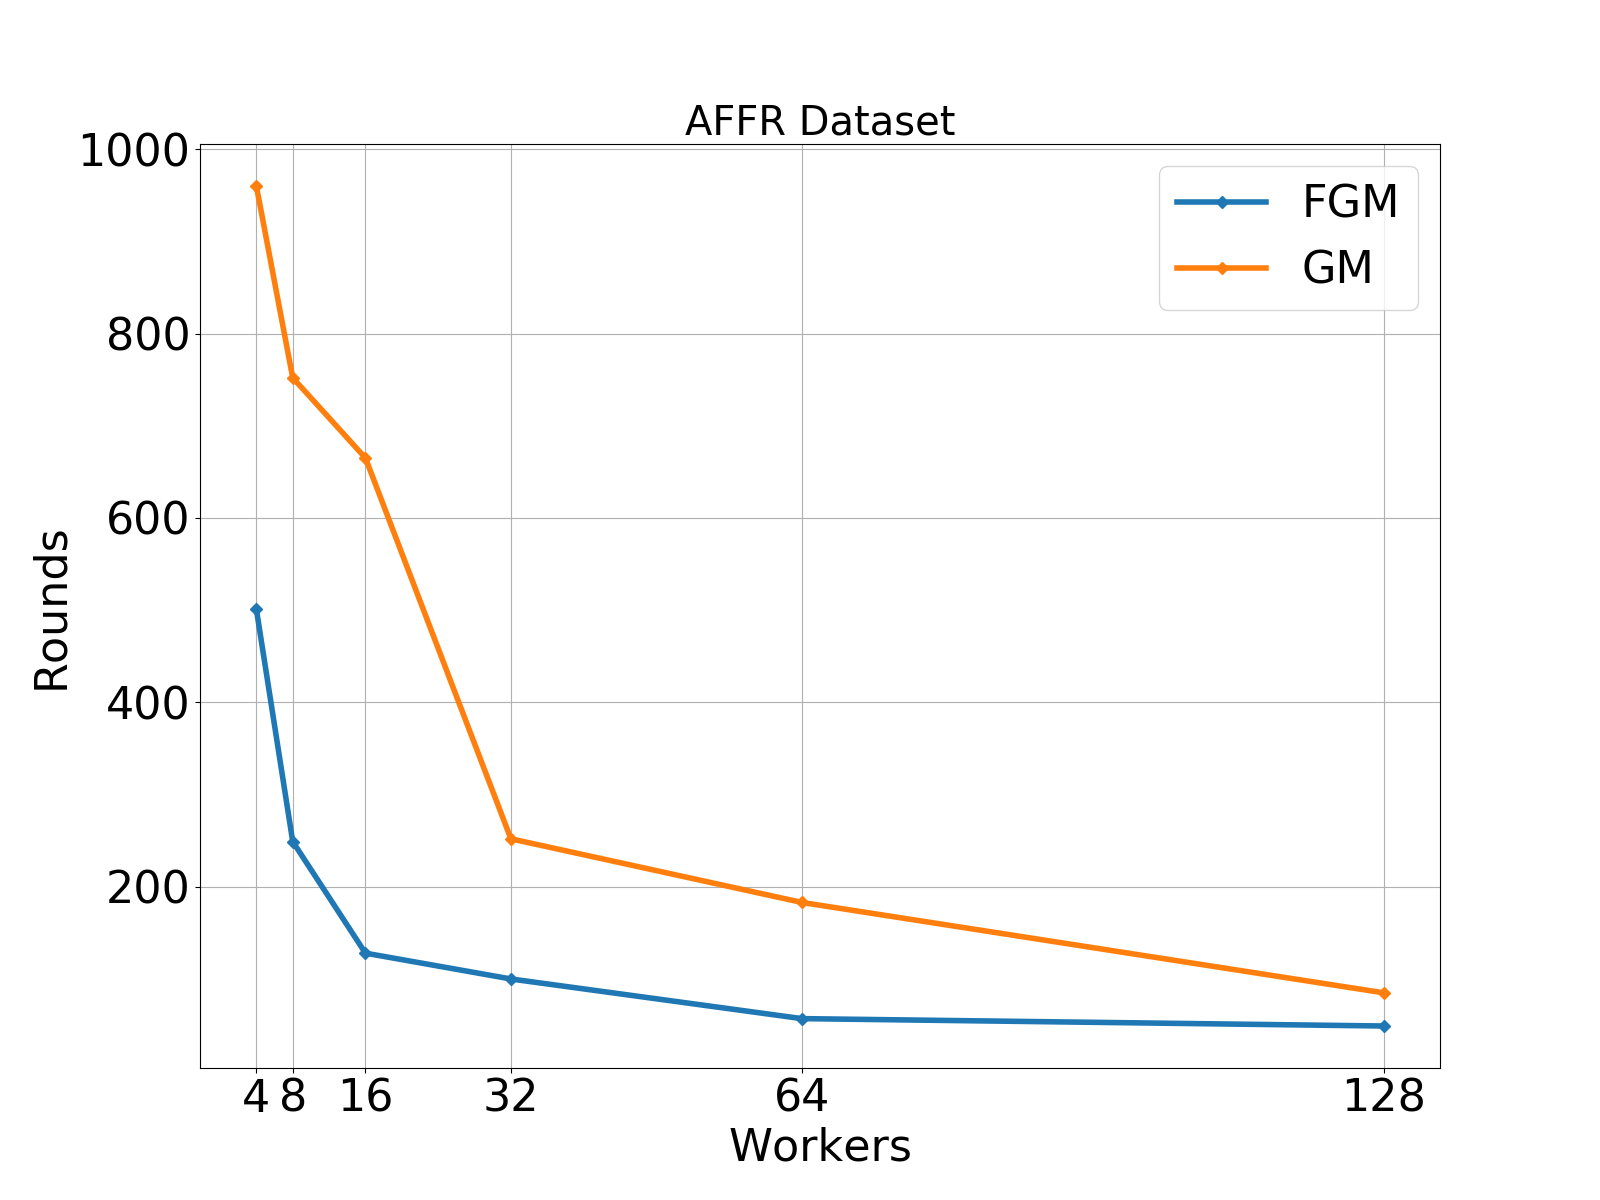
\includegraphics[width=3.9cm,height=3.5cm]{./images/results/amazon-plots/exp_Fig_3_2.png}}
        \subfigure{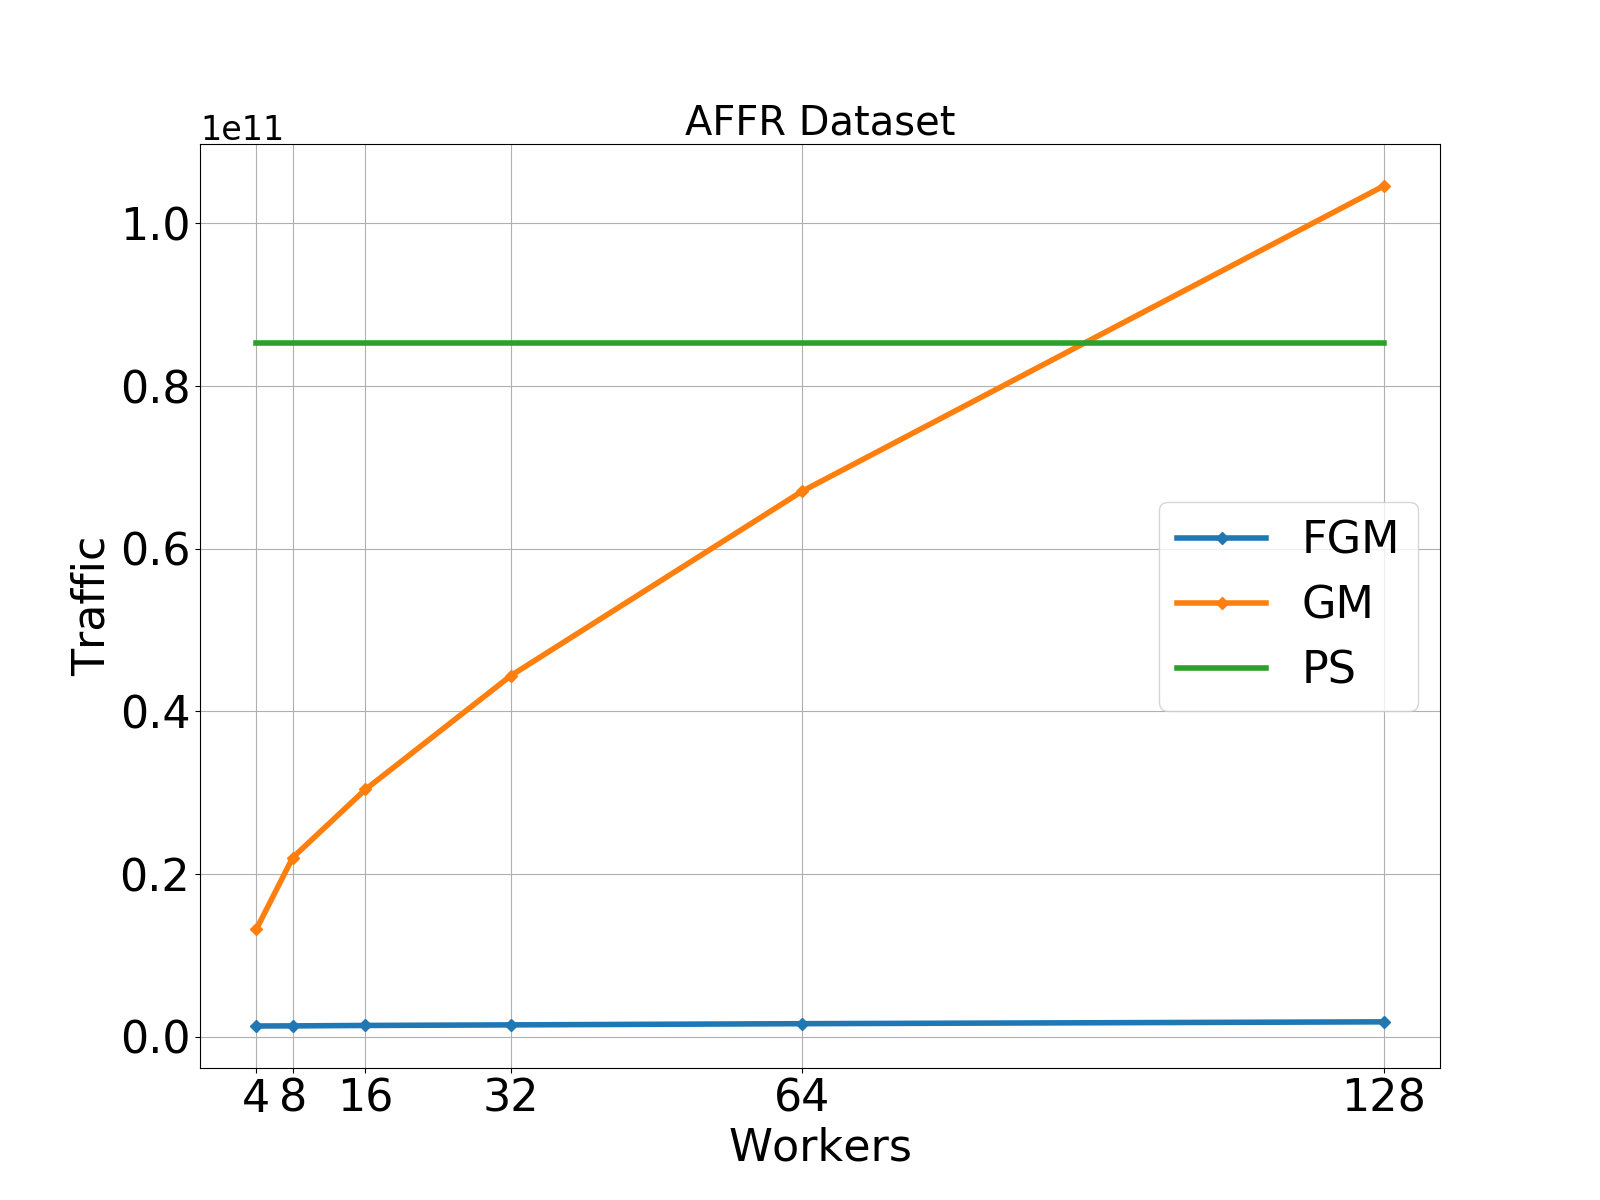
\includegraphics[width=3.9cm,height=3.5cm]{./images/results/amazon-plots/exp_Fig_3_3.png}}
        \label{fig:sfc-amazon-workers}
    \end{figure}
\end{frame}

\begin{frame}{Results (4) - Focusing on a specific case}
%    \begin{itemize}
%        \item{A comment.}
%    \end{itemize}
%    \vspace{-0.35cm}
    \begin{figure}
        \subfigure{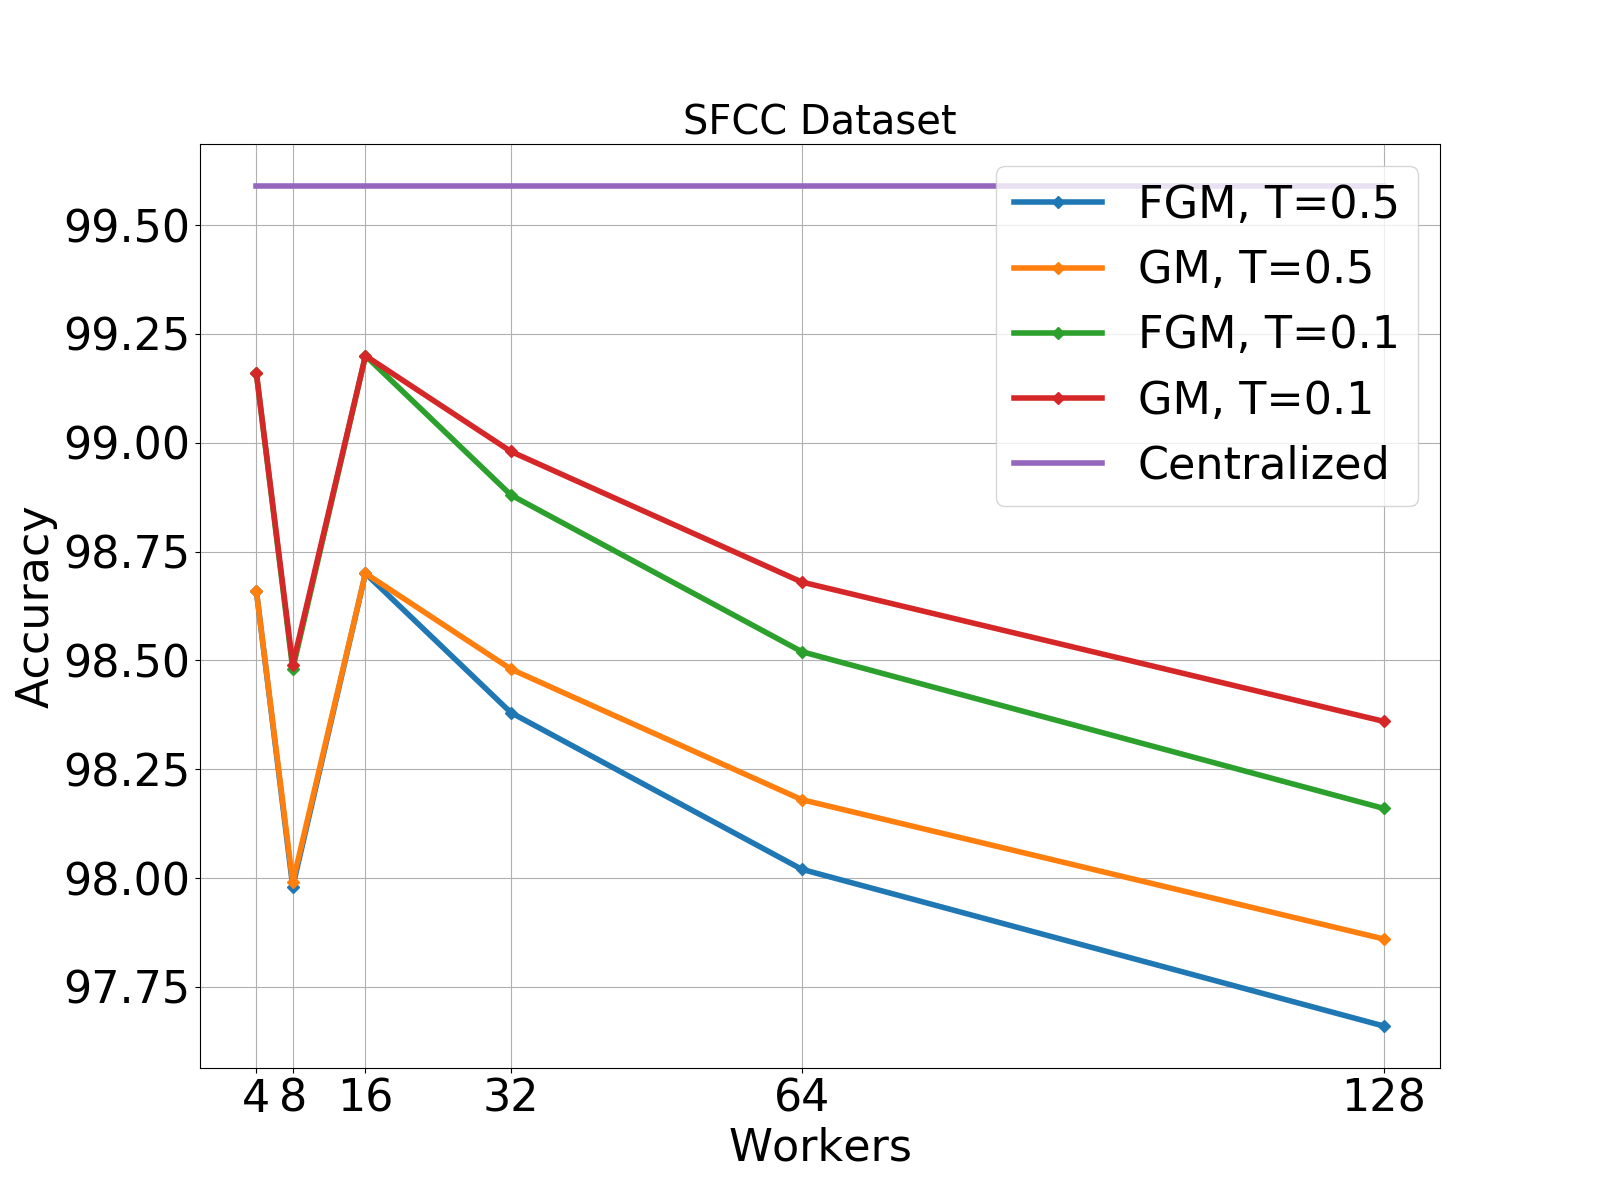
\includegraphics[width=5.2cm,height=3.7cm]{./images/results/sfc-plots/exp_Fig_3_1_b.png}}
        \subfigure{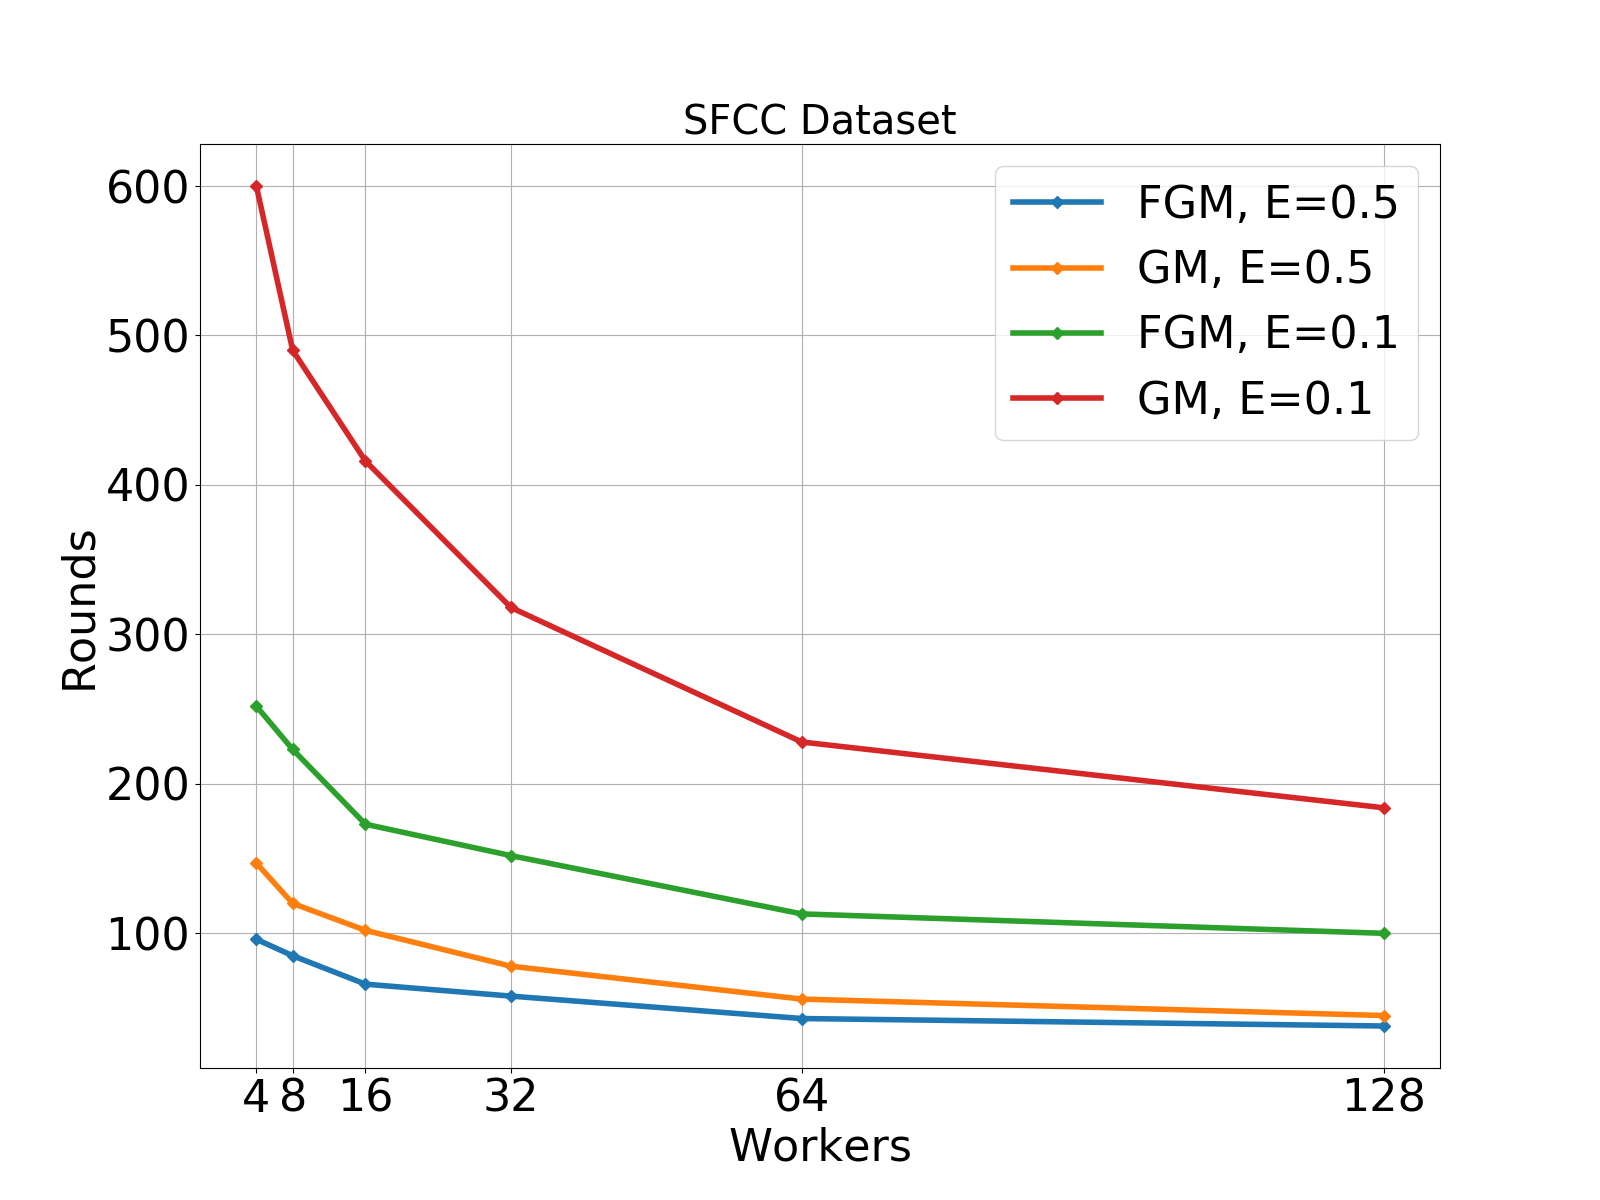
\includegraphics[width=5.2cm,height=3.7cm]{./images/results/sfc-plots/exp_Fig_3_2_b.png}}
        \subfigure{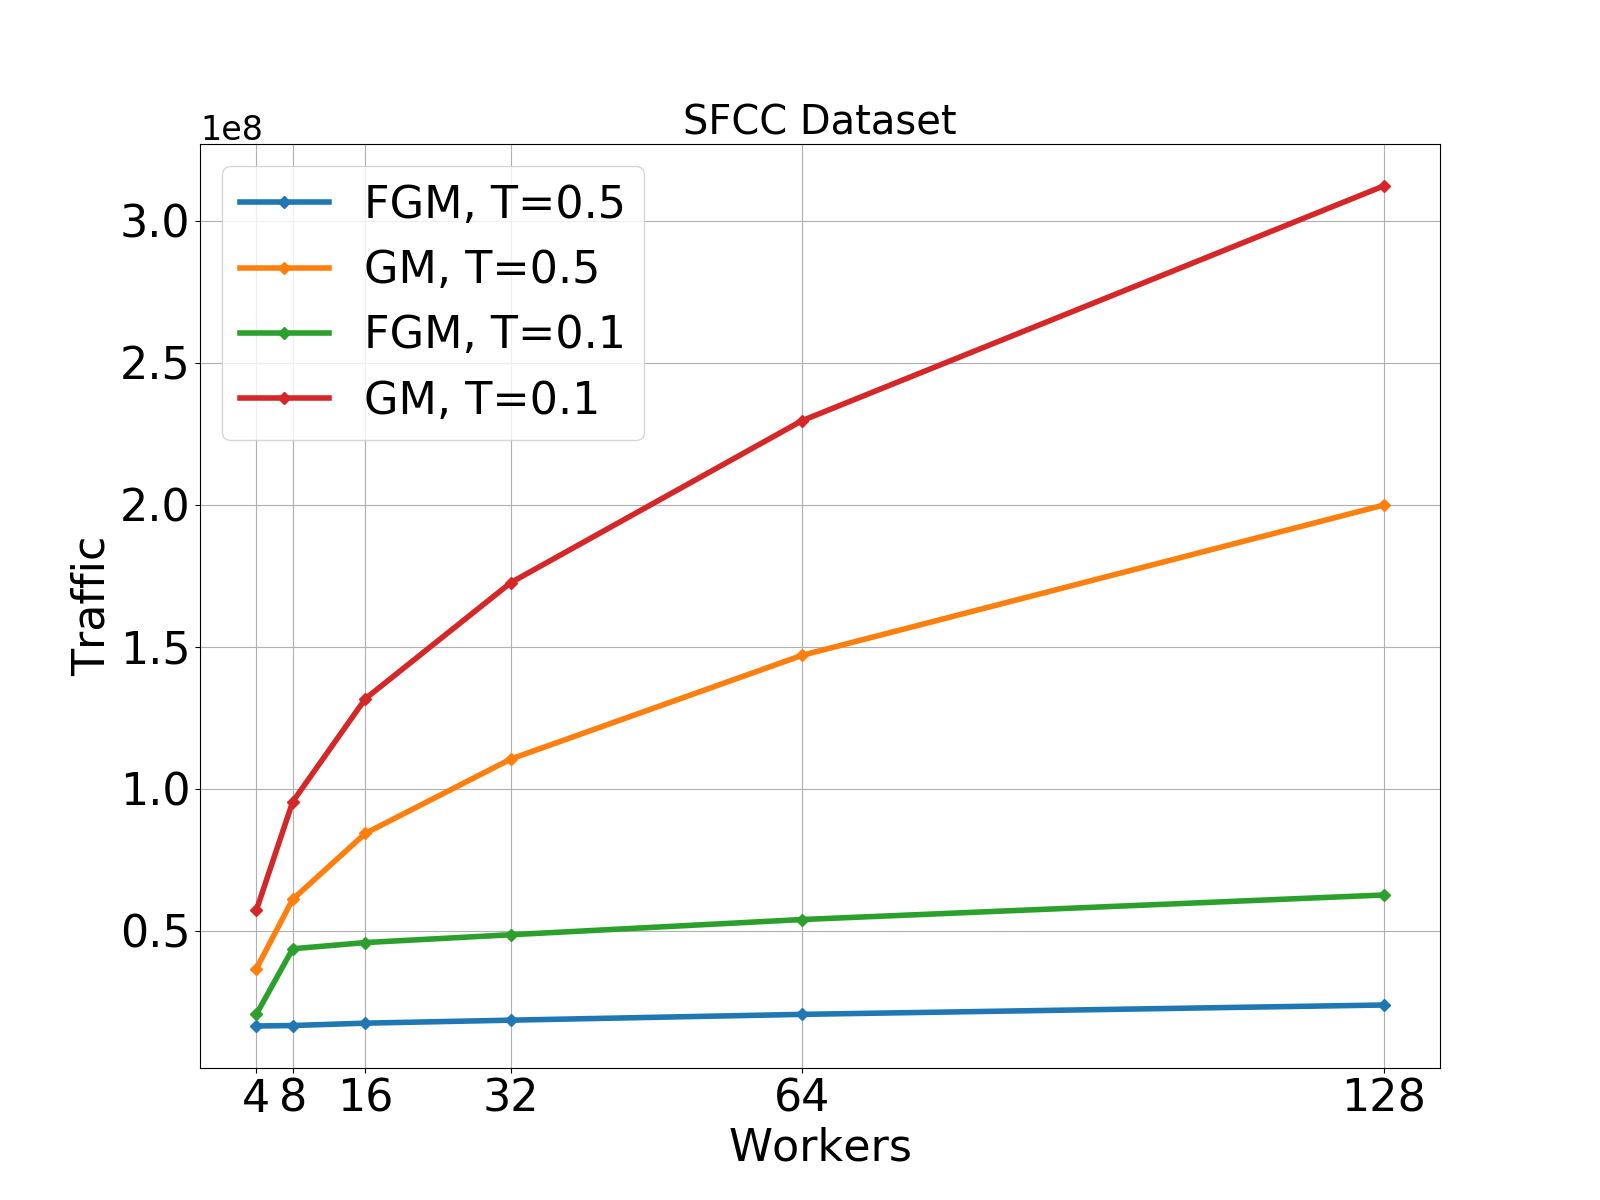
\includegraphics[width=5.2cm,height=3.7cm]{./images/results/sfc-plots/exp_Fig_3_3_b.png}}
        \label{fig:sfc_thres_workers}
    \end{figure}
\end{frame}

\subsection{Safe Functions Comparison}\label{subsec:safe-functions-comparison}

\begin{frame}{Safe Zone Problem}
    \setbeamertemplate{itemize items}[circle]
    \begin{itemize}
        \item{This time, we compare the two safe functions using the\\ \emph{same} protocol (\textbf{FGM}).}
        \item{The two safe functions are,}
        \vspace{0.2cm}
        \item[]{
        \begin{block}{Safe Function 1 (SF1) - \emph{'Simple norm'}}
            $\phi(\pmb{X_i},\pmb{E}) = ||\pmb{X_i}-\pmb{E}||_2^2 - T$
        \end{block}}
        \vspace{0.3cm}
        \begin{block}{Safe Function 2 (SF2) - \emph{'Spherical cap'}}
            $\phi(\pmb{X_i},\pmb{E}) = \max\{-T||\pmb{E}|| - \pmb{X_i}\frac{\pmb{E}}{\pmb{||E||}}, ||\pmb{X_i}+\pmb{E}|| - (1+T)||\pmb{E}||\}$
        \end{block}
    \end{itemize}
\end{frame}

\begin{frame}{Results (1) - Accuracy}
    \setbeamertemplate{itemize items}[circle]
    \begin{itemize}
        \item{\textbf{SF1} achieves a little bit \textbf{better} accuracy.}
    \end{itemize}
    \vspace{-0.35cm}
    \begin{figure}
        \subfigure{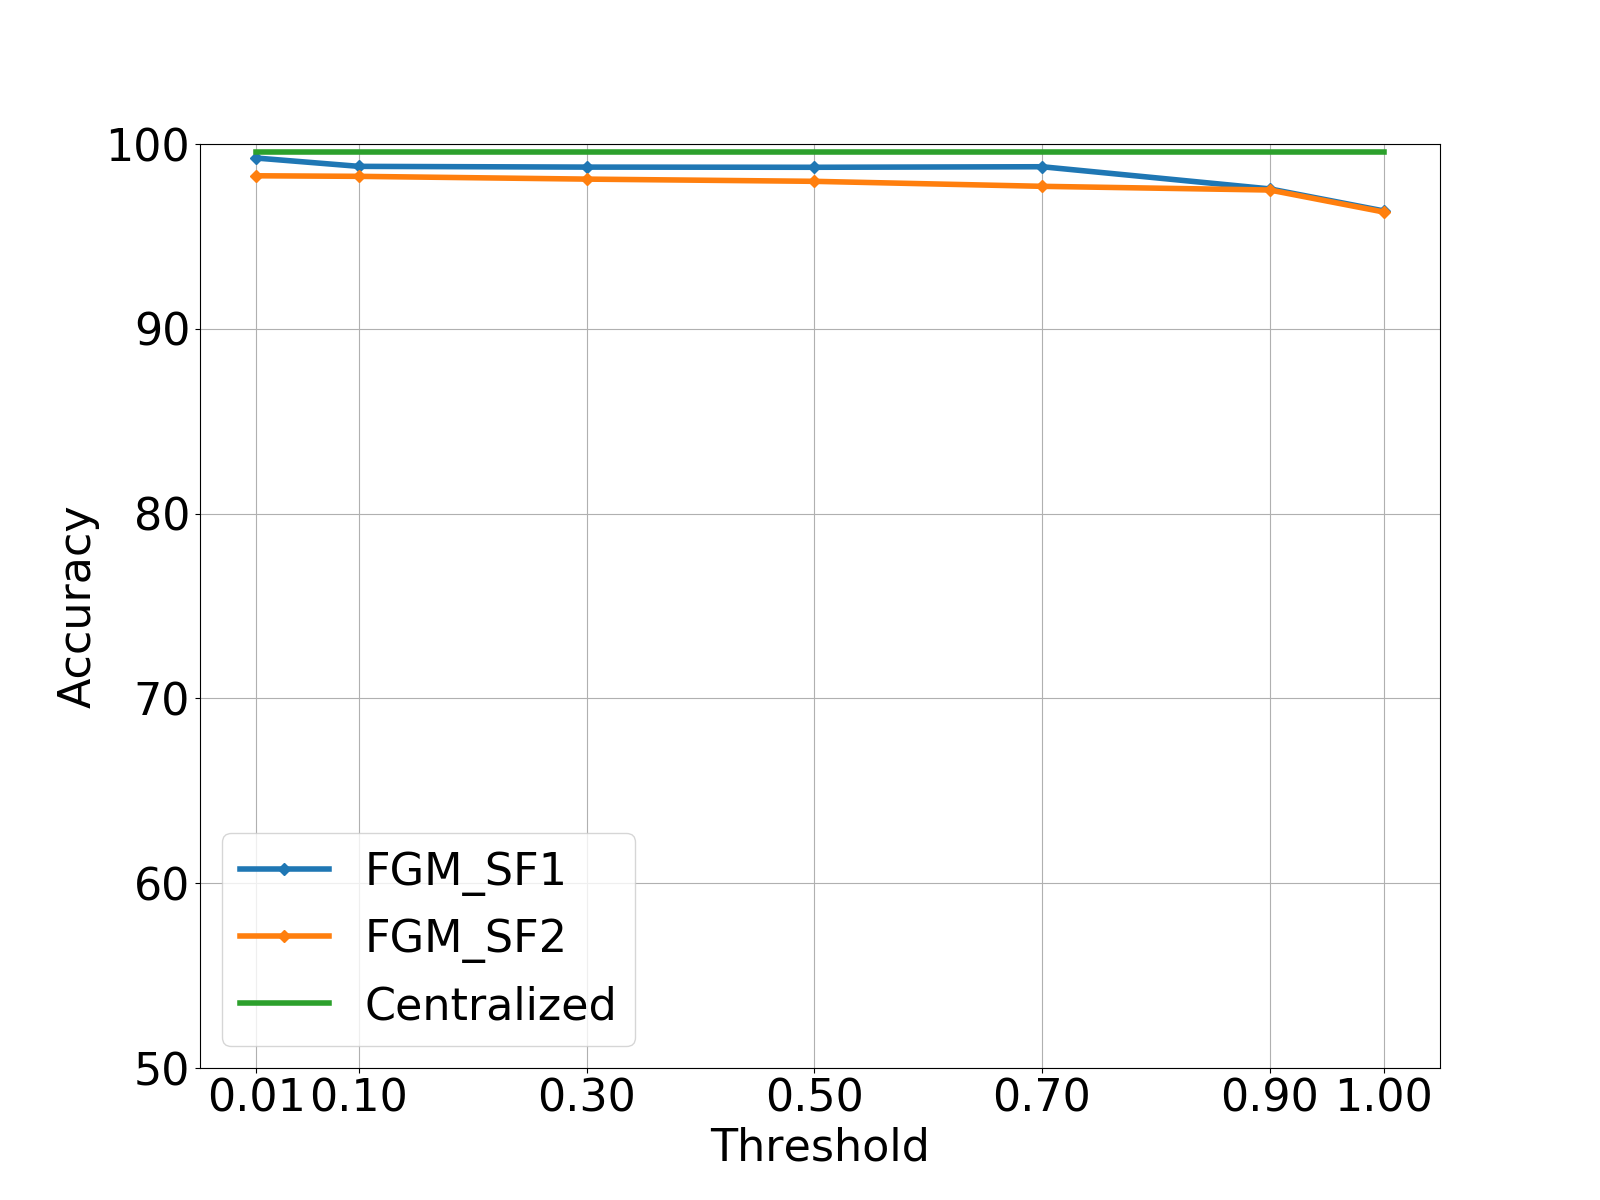
\includegraphics[width=5.2cm,height=3.7cm]{./images/results/sf-comp/exp_Fig_1_1.png}}
        \subfigure{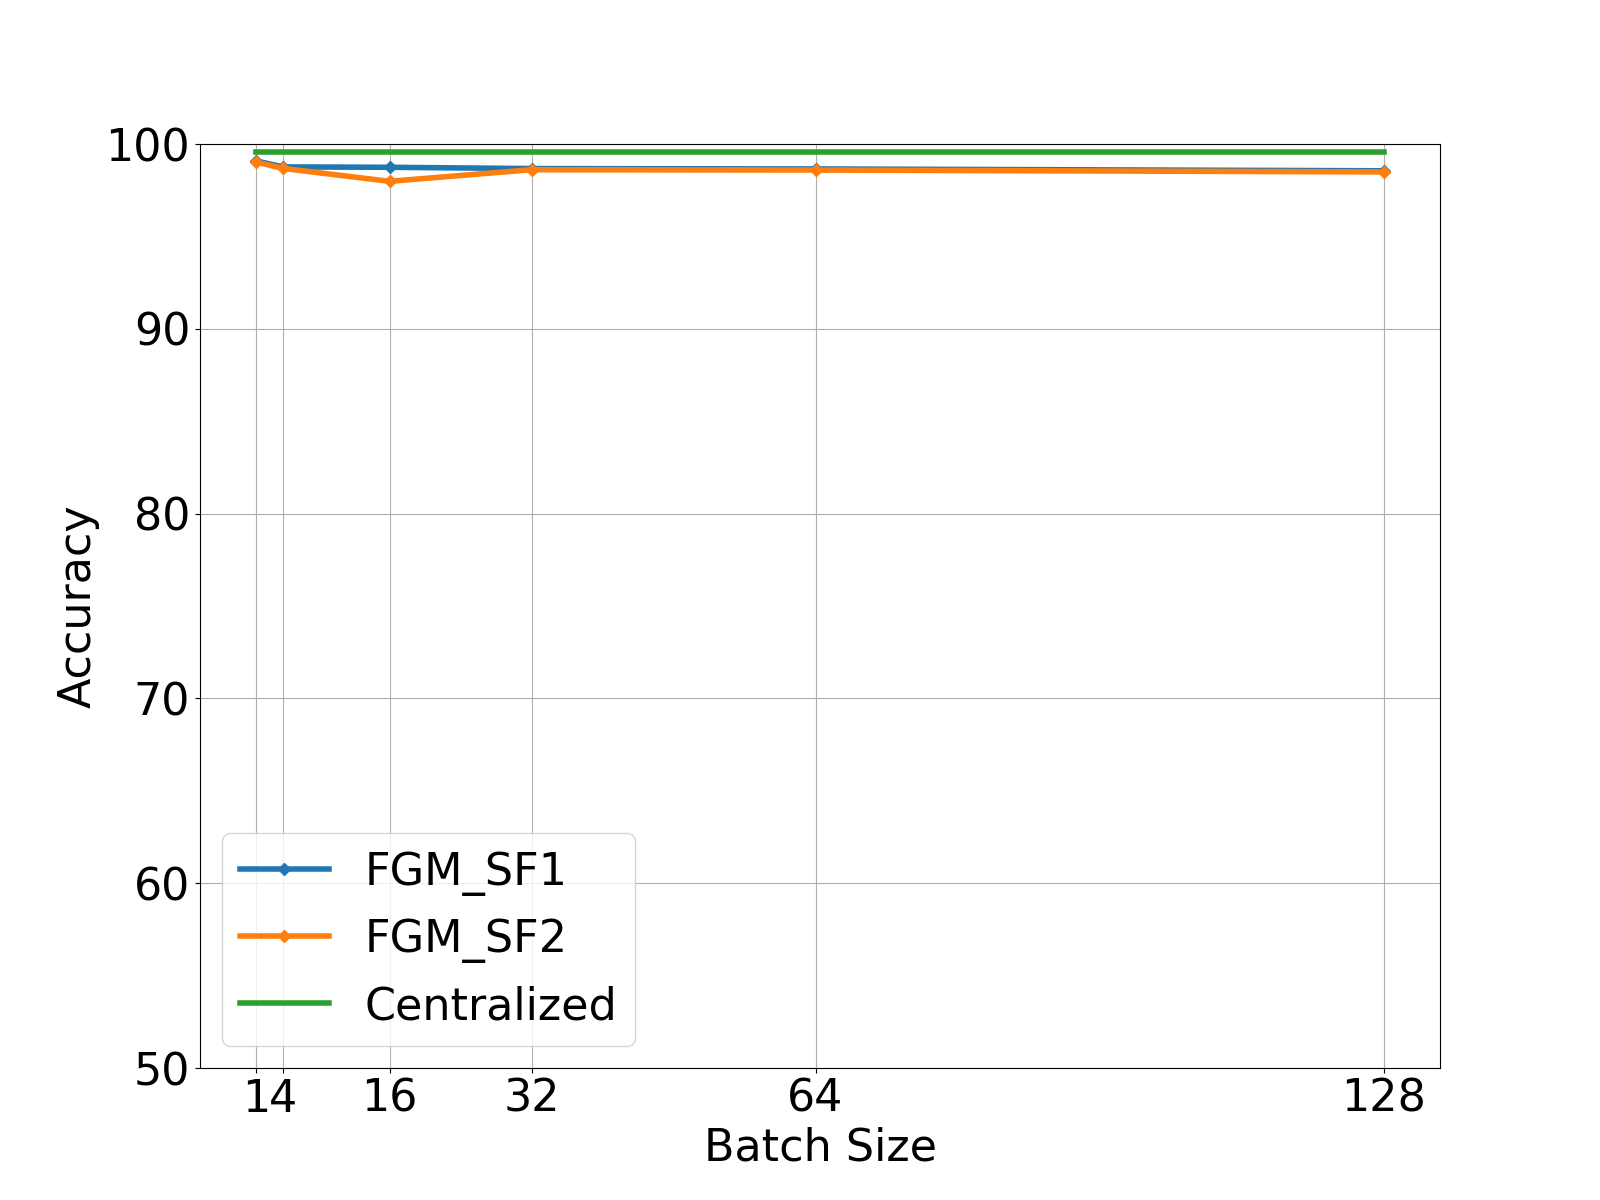
\includegraphics[width=5.2cm,height=3.7cm]{./images/results/sf-comp/exp_Fig_2_1.png}}
        \subfigure{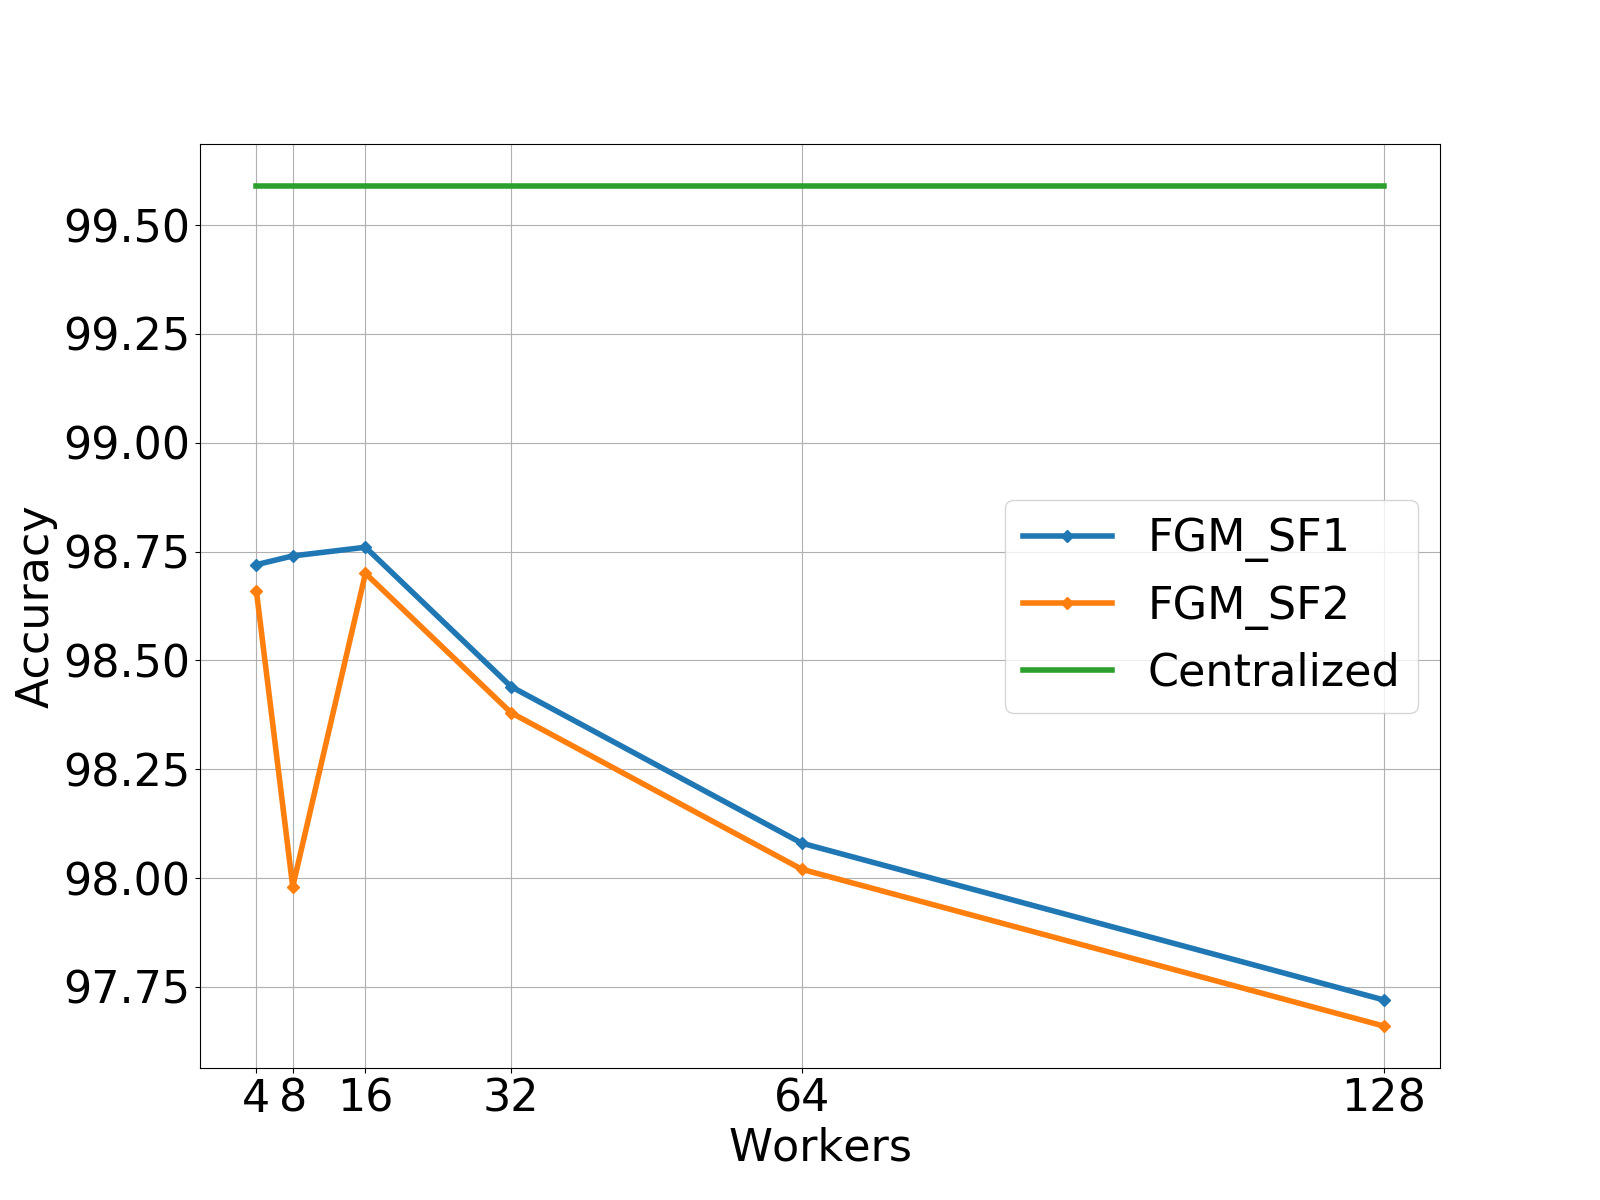
\includegraphics[width=5.2cm,height=3.7cm]{./images/results/sf-comp/exp_Fig_3_1.png}}
        \label{fig:sf_acc}
    \end{figure}
\end{frame}

\begin{frame}{Results (2) - Number of rounds}
%    \setbeamertemplate{itemize items}[circle]
%    \begin{itemize}
%        \item{A comment}
%    \end{itemize}
%    \vspace{-0.35cm}
    \begin{figure}
        \subfigure{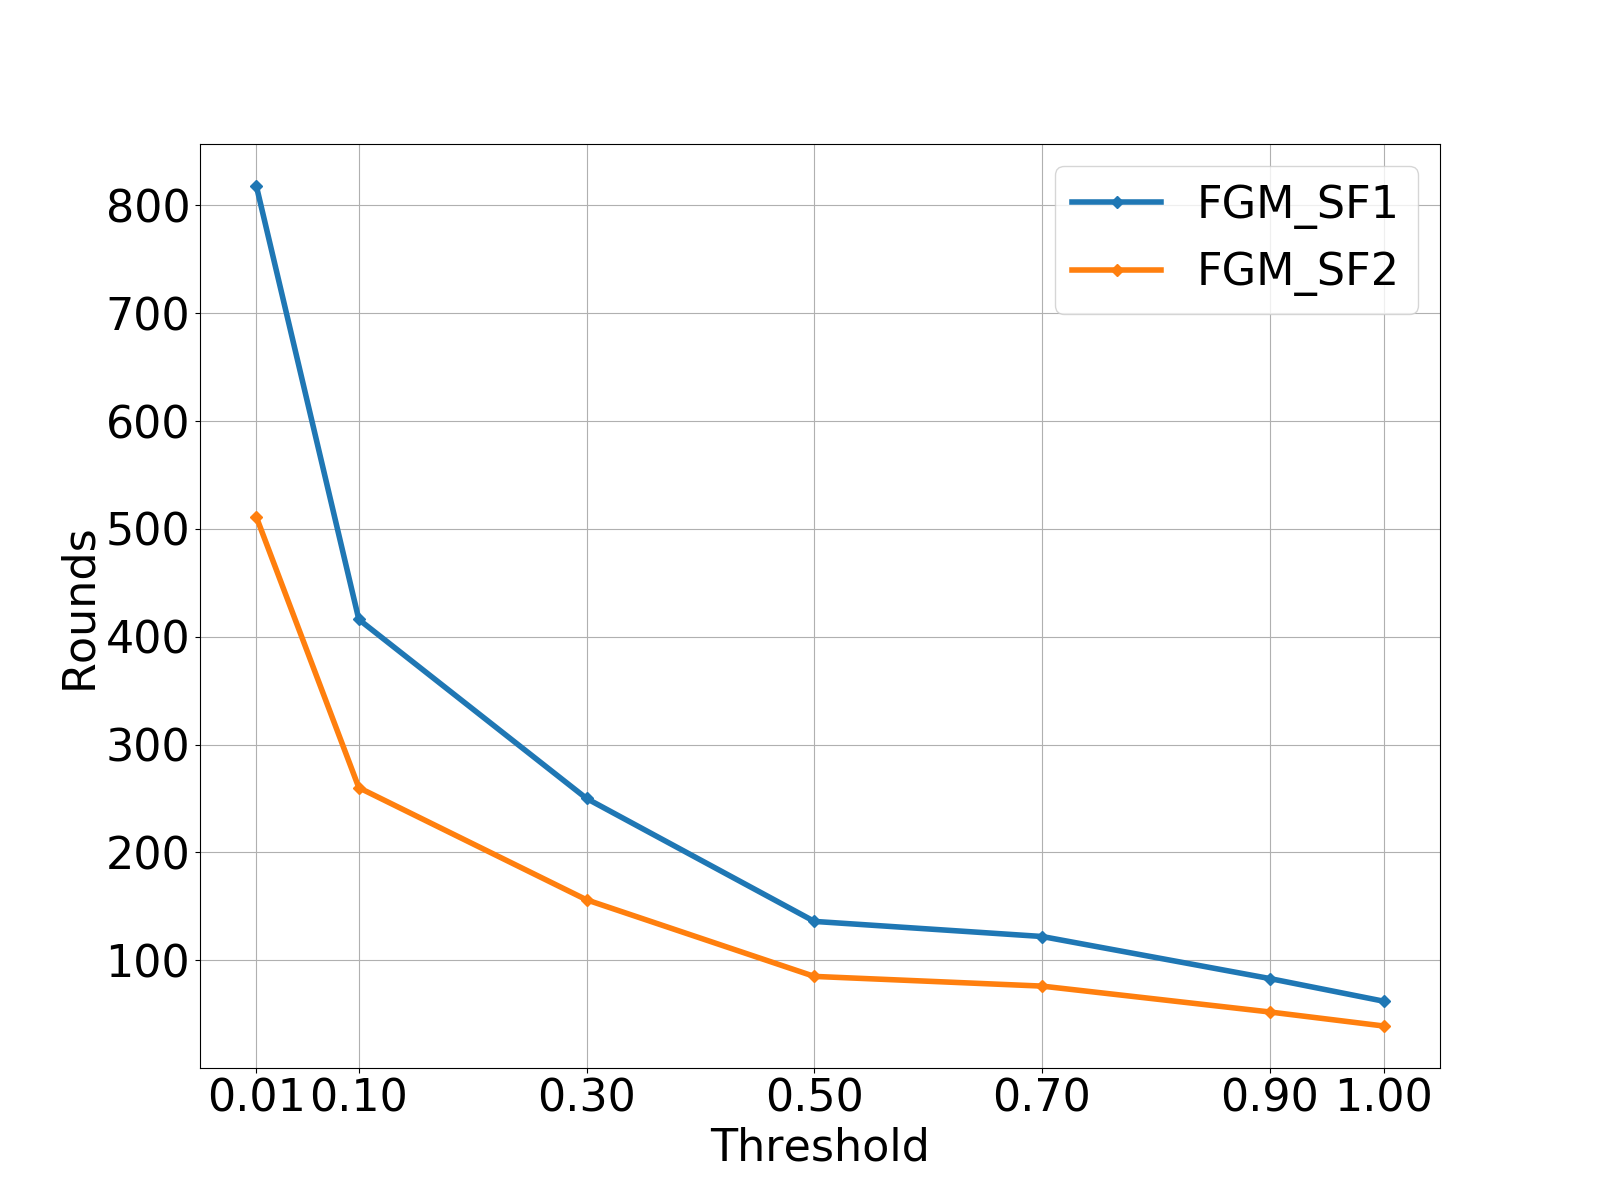
\includegraphics[width=5.2cm,height=3.7cm]{./images/results/sf-comp/exp_Fig_1_2.png}}
        \subfigure{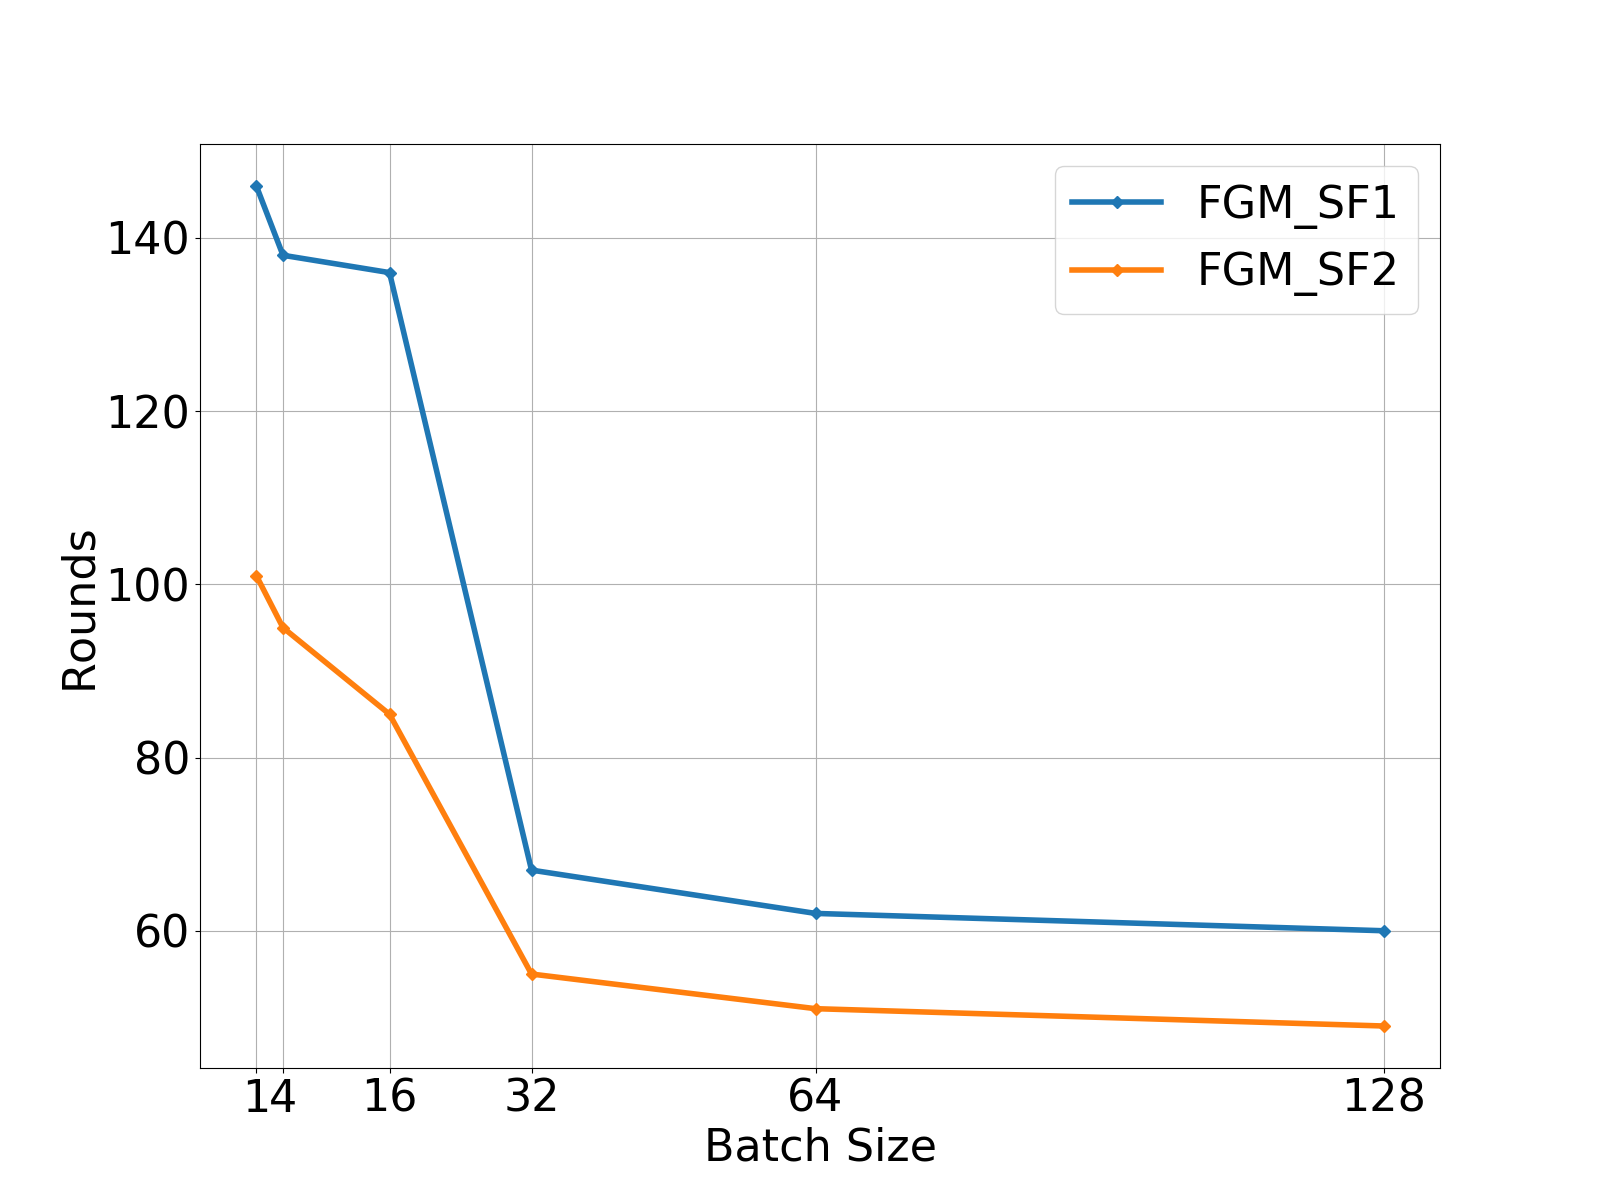
\includegraphics[width=5.2cm,height=3.7cm]{./images/results/sf-comp/exp_Fig_2_2.png}}
        \subfigure{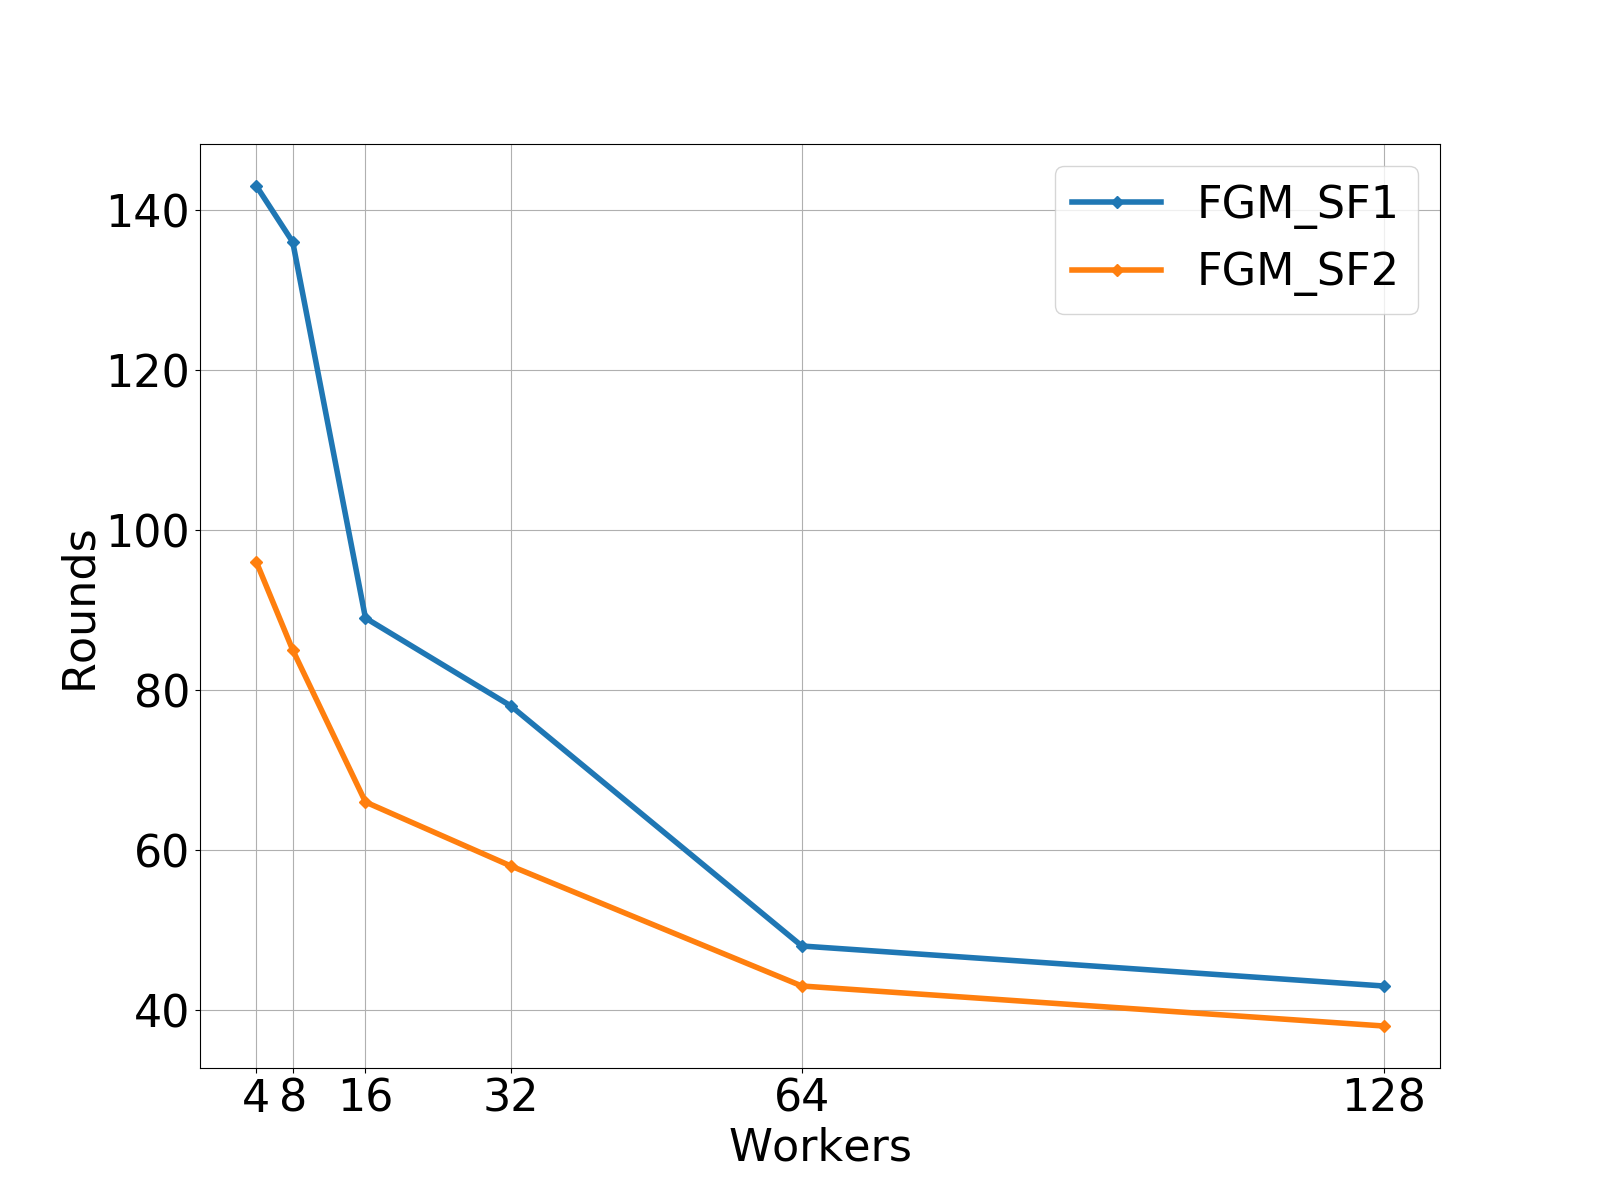
\includegraphics[width=5.2cm,height=3.7cm]{./images/results/sf-comp/exp_Fig_3_2.png}}
        \label{fig:sf_rnds}
    \end{figure}
\end{frame}

\begin{frame}{Results (3) - Scalabilty Analysis}
    \setbeamertemplate{itemize items}[circle]
    \begin{itemize}
        \item{\textbf{SF2} is more \textbf{efficient} by up to 56\%.}
    \end{itemize}
    \vspace{-0.35cm}
    \begin{figure}
        \subfigure{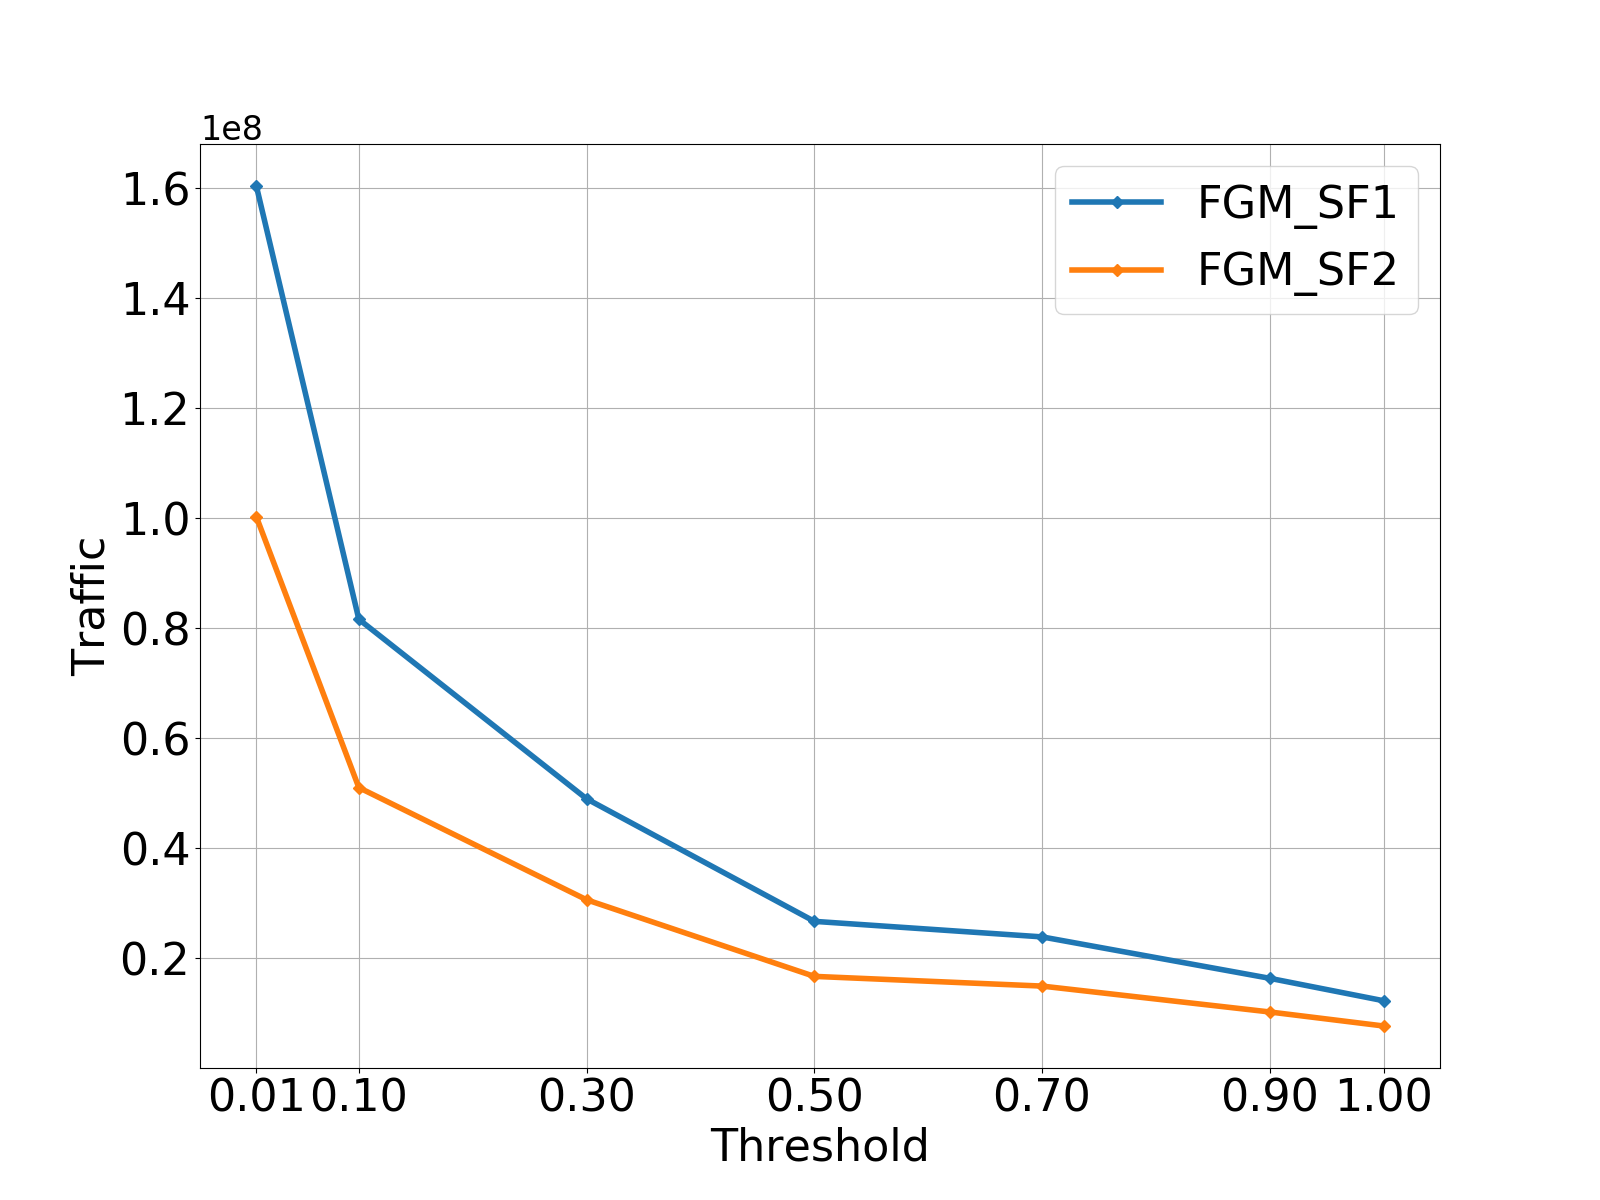
\includegraphics[width=5.2cm,height=3.7cm]{./images/results/sf-comp/exp_Fig_1_3.png}}
        \subfigure{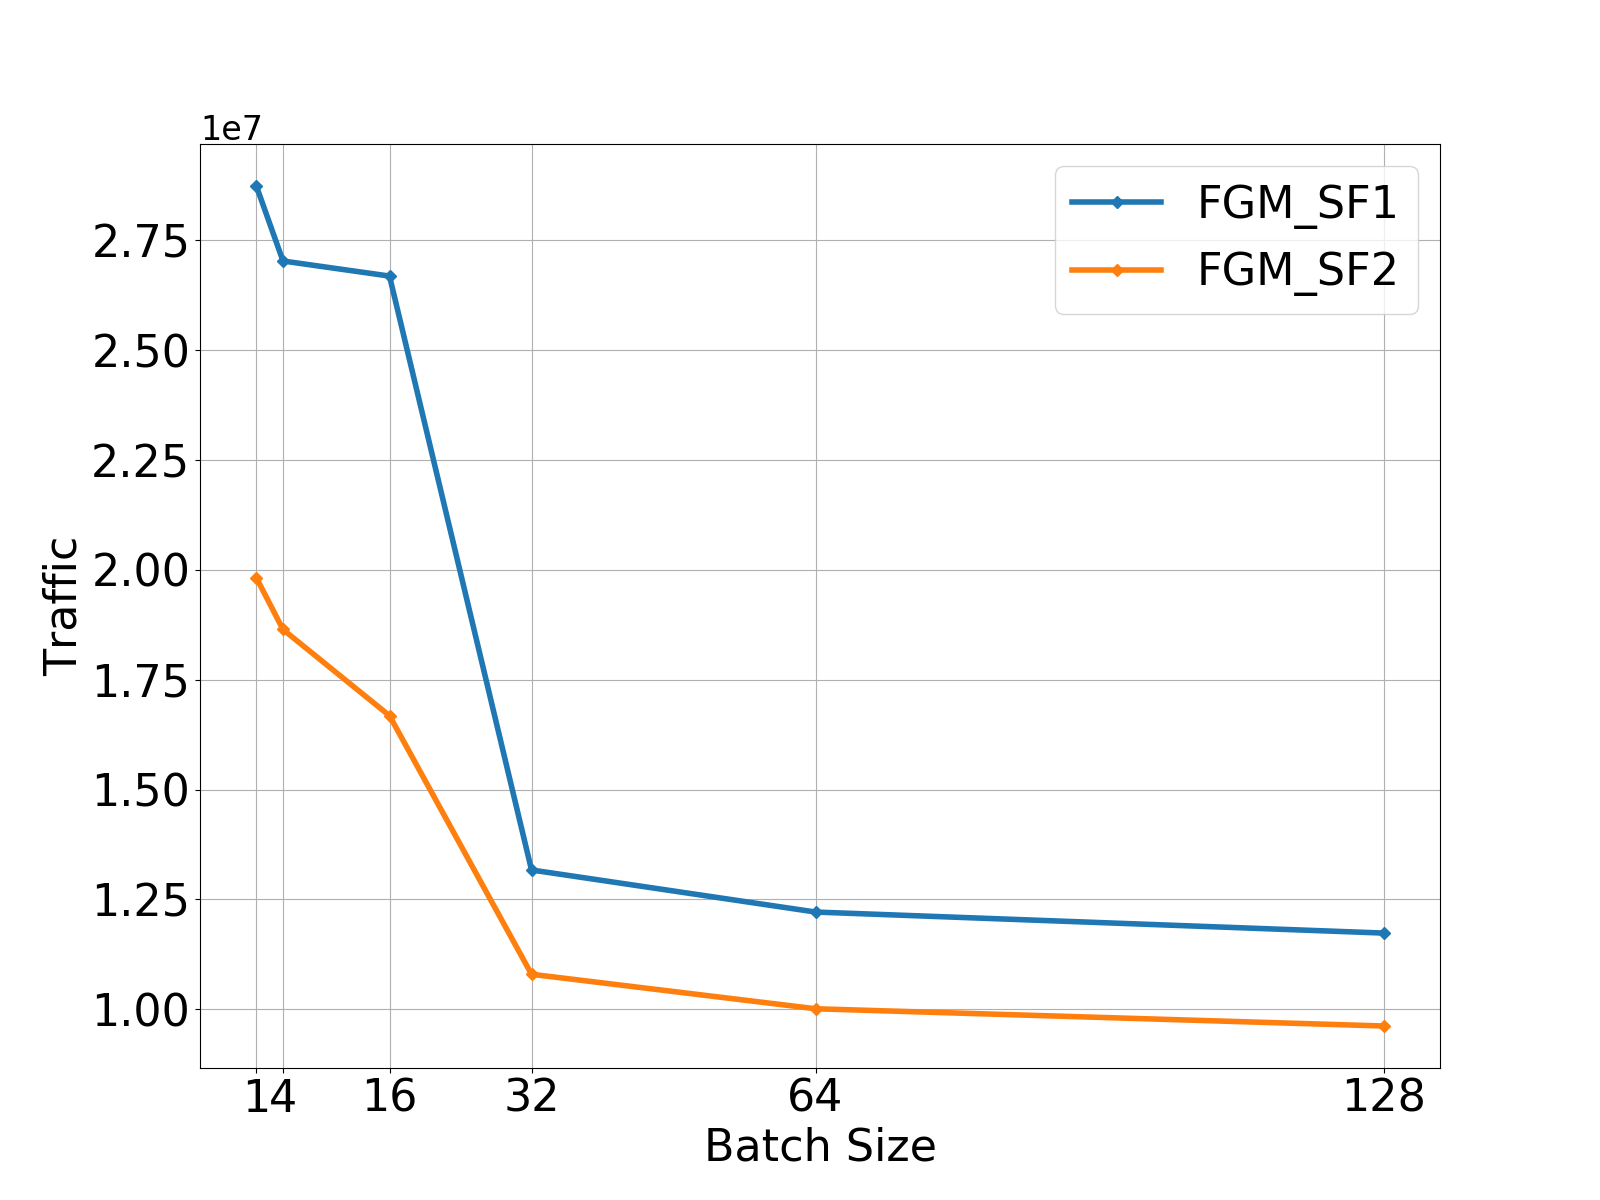
\includegraphics[width=5.2cm,height=3.7cm]{./images/results/sf-comp/exp_Fig_2_3.png}}
        \subfigure{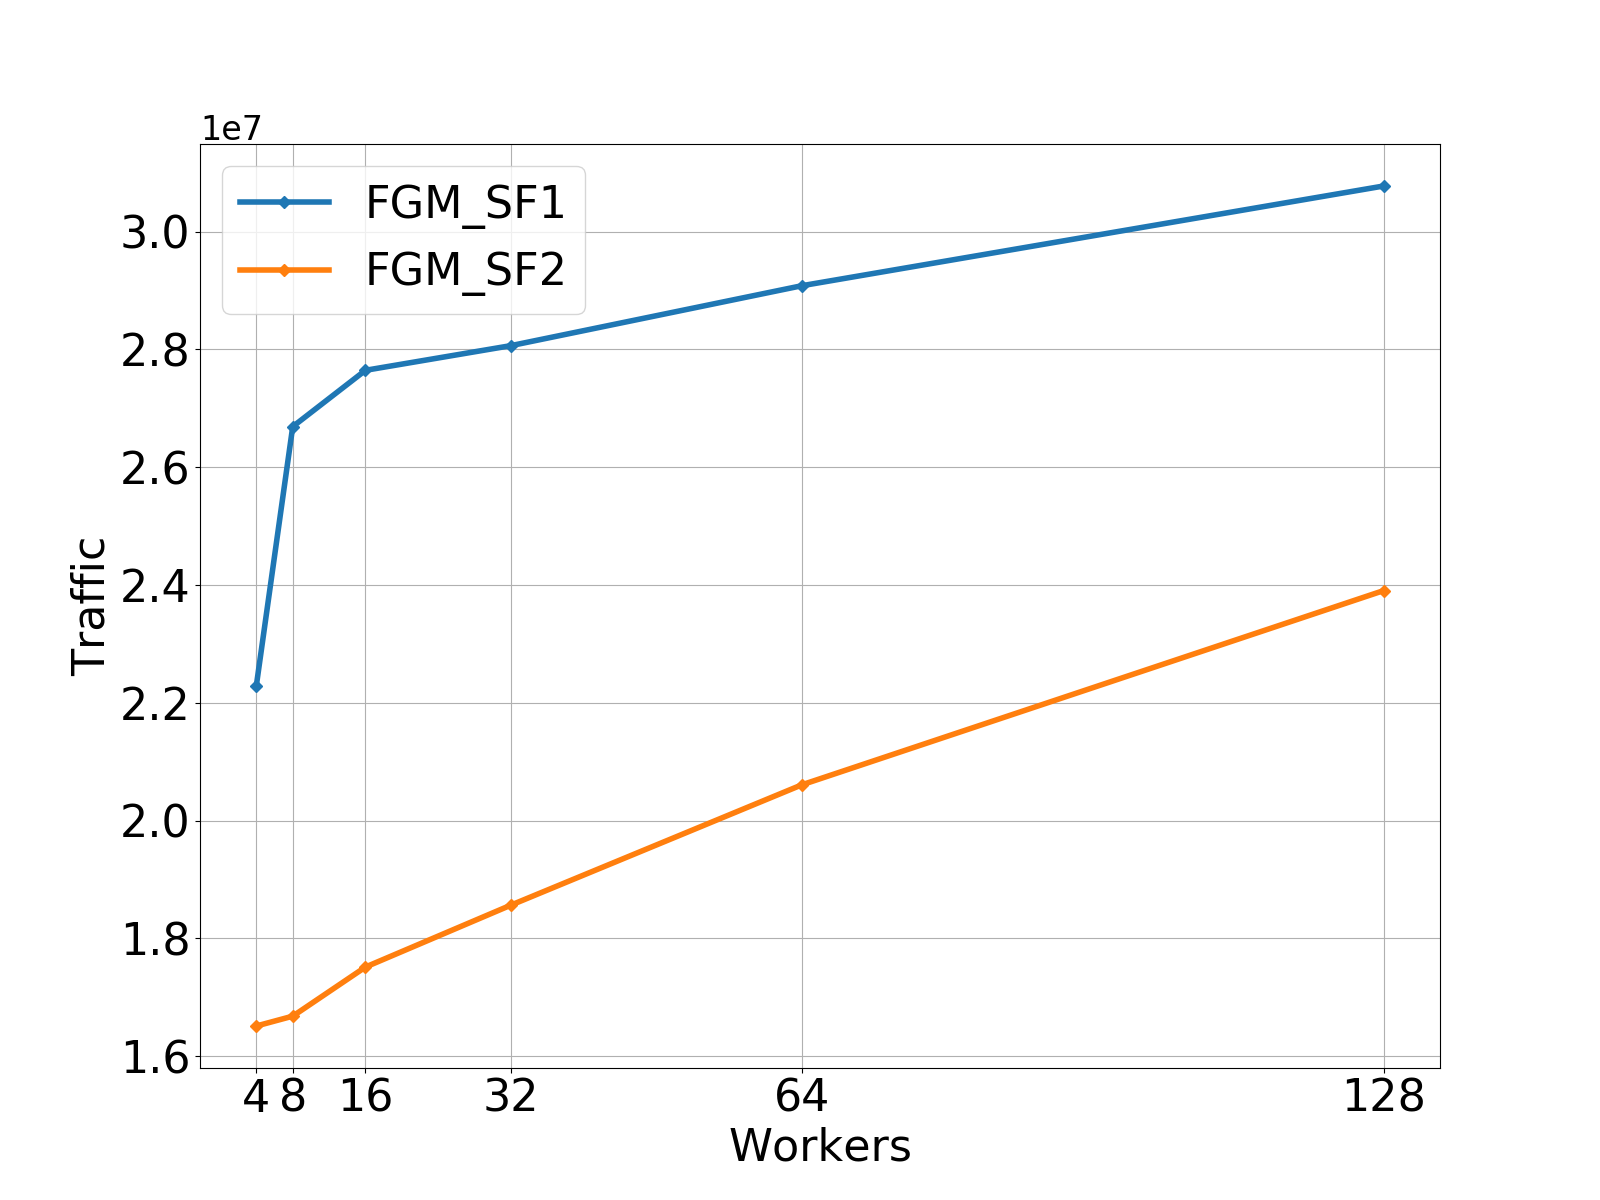
\includegraphics[width=5.2cm,height=3.7cm]{./images/results/sf-comp/exp_Fig_3_3.png}}
        \label{fig:sf_trff}
    \end{figure}
\end{frame}